\documentclass{beamer}


% Setup appearance:

\usetheme{Darmstadt}
\usefonttheme[onlylarge]{structurebold}
\setbeamerfont*{frametitle}{size=\normalsize,series=\bfseries}
\setbeamertemplate{navigation symbols}{}


% Standard packages

\usepackage[spanish]{babel}
\usepackage[latin1]{inputenc}
\usepackage{times}
\usepackage[T1]{fontenc}


% Setup TikZ

\usepackage{tikz}
\usetikzlibrary{arrows}
\tikzstyle{block}=[draw opacity=0.7,line width=1.4cm]


% Author, Title, etc.

\title[Block Partitioning and Perfect Phylogenies] 
{ Estudios de simulación en la búsqueda de nuevos bosones ligeros durante la fase de alta luminosidad del experimento CMS del CERN.
}

\author[Lic. Francisco Martínez Sánchez]
{  Autor: Lic. Francisco Martínez Sánchez

Miembros del comité:

Alfredo Martín Castañeda Hernandez (Director)

Susana Alvarez Garcia (tutor)

Marcelino Barbosa Flores (tutor)}

\institute[]
{
  Reporte Avance de Tesis, Universidad de Sonora, Hermosillo, Sonora 2020
}




% The main document

\begin{document}

\begin{frame}
  \titlepage
\end{frame}

\begin{frame}{Outline}
  \tableofcontents
\end{frame}


%\section{Motivacion}
\section{Introduccion}
%\input{Introduccion}




\section{Simulación}
%\begin{frame}{}
    \begin{center}
        \LARGE Simulación
    \end{center}
\end{frame}

\begin{frame}{Simulación}

\begin{itemize}
    \item Para estudiar el modelo Dark-SUSY de forma experimental y caracterizar las propiedad de la se\~nal  
    se requiere generar muestras de simulación por el método de Monte Carlo 
    \item La simulación requiere generar varias muestras considerando los parámetros m\'as importantes del fotón oscuro (masa y tiempo de vida) 
    \item Para generar las muestras simuladas se hace uso de paquetes propios del área de altas energías, los cuales actúan de forma sequencial y se encargan de diferentes aspectos del proceso de análisis. 
\end{itemize}
    
\end{frame}


\begin{frame}{Paquetes de Simulación}
\begin{itemize}
    \item \textbf{Madgraph}: Se encarga de procesar la informaci\'on fundamental del modelo como la masa de las particulas madre, diagramas de Feynman, amplitudes de decaimiento, etc. 
    \item \textbf{Pythia}: Se encarga del proceso de hadronización, es decir la interacción entre protones, recombinación de quarks y formación de nuevas partículas 
    \item \textbf{Delphes}: Se encarga de simular la respuesta del detector al paso de las partículas simuladas, en este paso se consideran eficiencia de detecciones y se extraen variables como la energia, momento y trayectoria reconstruida de las partículas en cuestión
\end{itemize}

\end{frame}

\begin{frame}{Estrategia de Simulación}

\begin{itemize}
    \item Para generar las muestras se requiere crear un entorno automatizado (python) el cual pueda ser flexible a las diferentes variaciones del modelo
    \item Los archivos resultantes (formato .root) contienen la informaci\'on (teorica+experimental) para realizar el an\'alisis de datos.  
\end{itemize}

\begin{figure}[h]
\centering
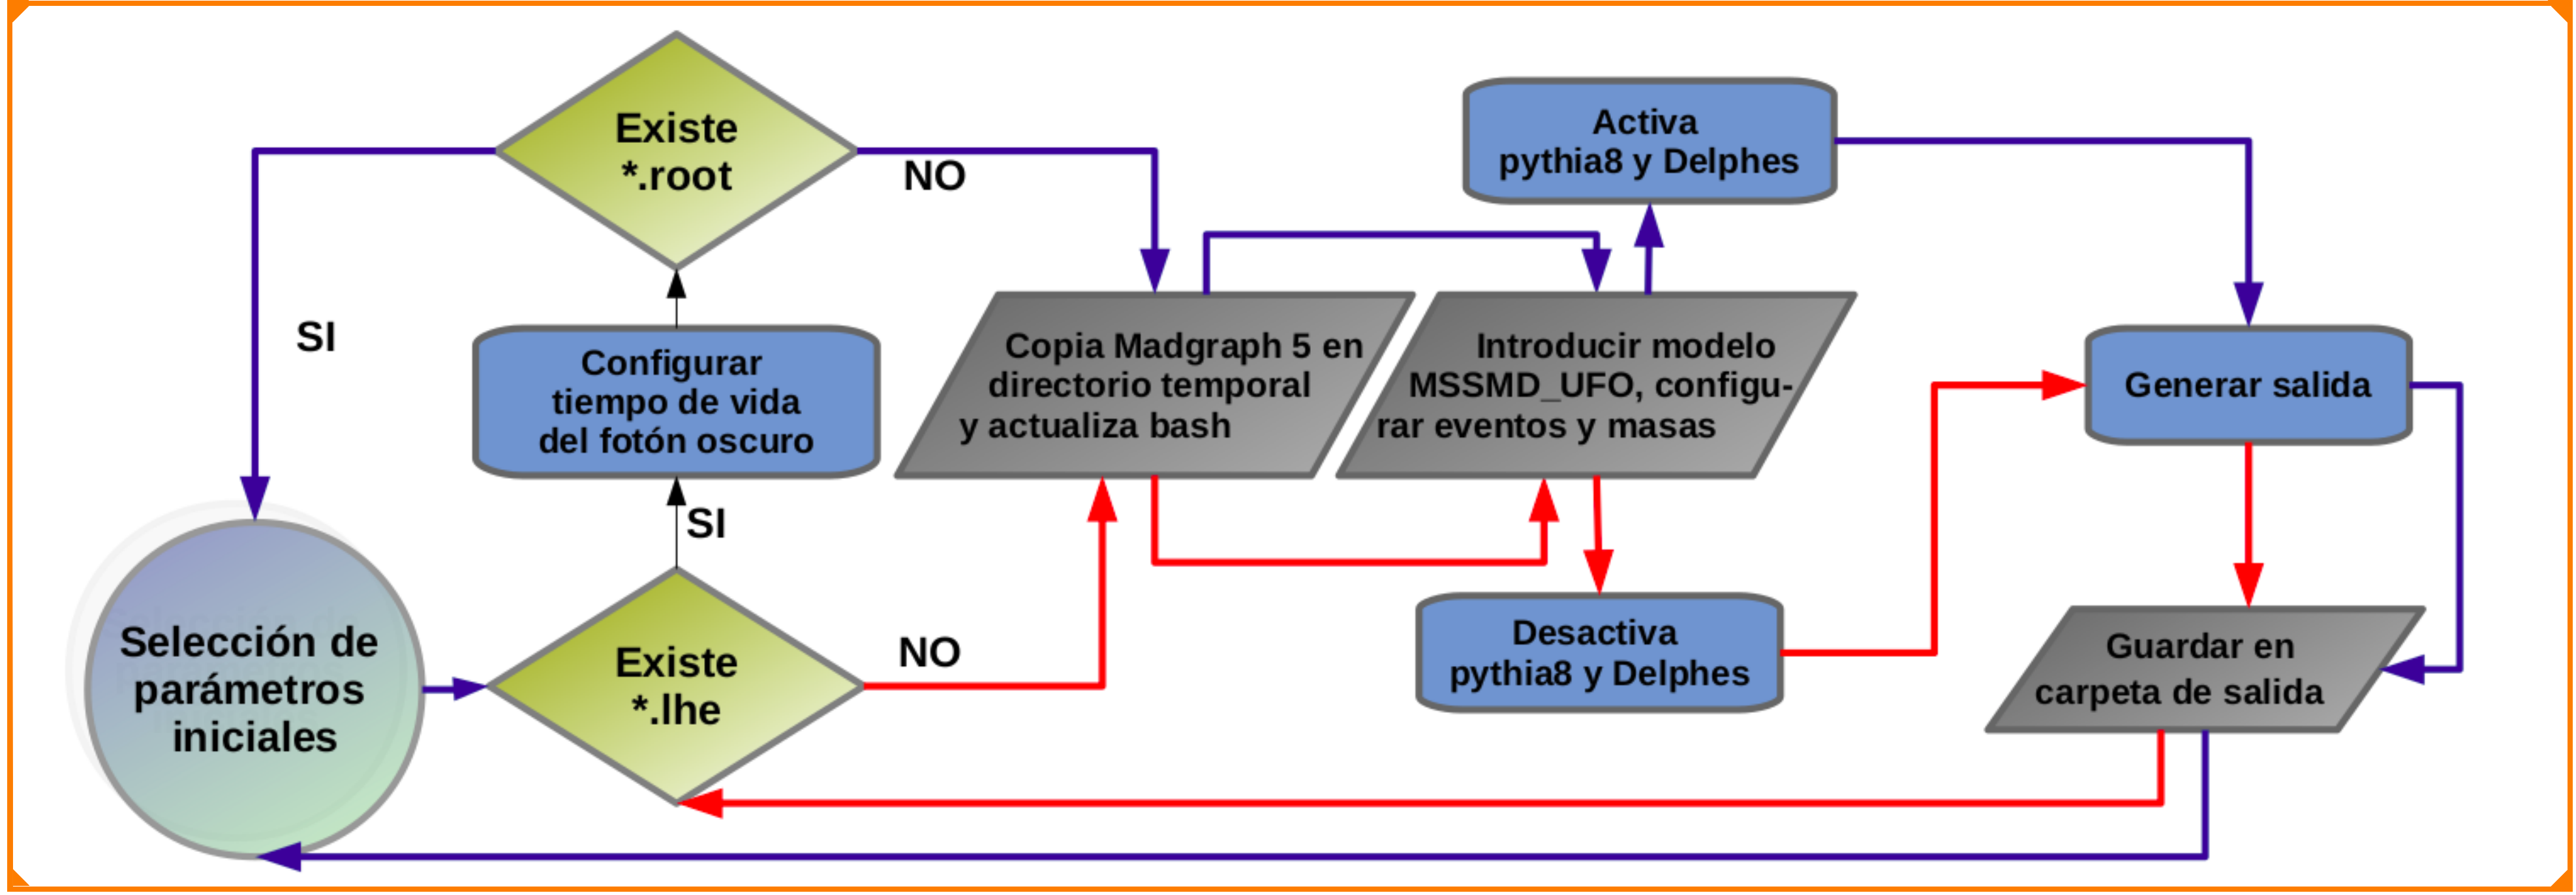
\includegraphics[width=0.8\textwidth]{Imag/proyecto_darksusy2.png}
\caption{Diagrama de Flujo del generador.}
\end{figure}

%Incluir diagrama donde se describa como se inicia la simulacion Madgraph->Pythia->Delphes
    
\end{frame}


\begin{frame}{Muestras simuladas}
    \begin{itemize}
        \item Para generar cada muestra se requiere especificar los siguientes parámetros: masa del neutralino ($m_{n_{1}}$), masa del dark neutralino ($m_{n_{D}}$), masa del fotón oscuro ($m_{\gamma_{D}}$) y tiempo de vida del foton oscuro ($c\tau_{\gamma_{D}}$) que son los parámetros del modelo Dark-SUSY. 
        %\item El numero de muestras simuladas se representa en la siguiente tabla
        \item El número de muestras simuladas es el resultado de todas las combinaciones posibles de los vectores correspondientes a los parámetros de generación, haciendo un total de $\backsim 15 000$ muestras:
    \end{itemize}

\begin{table}
\begin{footnotesize}
\begin{tabular}{|cl|}
\hline
$V_{m_{n_{1}}}$ & = $[10, ~20, ~30, ~40, ~50, ~60, ~70, ~80, ~90, ~100]$\\
$V_{m_{n_{D}}}$ & = $[0.25, ~1, ~2, ~3, ~4, ~5, ~10]$\\
$V_{m_{\gamma_{D}}}$ & = $[0.25, ~1, ~2, ~3, ~4, ~5, ~6, ~7, ~8, ~9, ~10]$\\
$V_{c\tau_{\gamma_{D}}}$ & = $[0, ~1, ~2, ~3, ~4, ~5, ~10, ~20, ~30, ~40, ~50, ~100]$\\
Eventos simulados &  = 10000\\
\hline
\hline
\end{tabular}
\end{footnotesize}
\end{table}

    
%\begin{table}
%\begin{footnotesize}
%\begin{tabular}{|ccccc|}
%\hline
%$m_{n_{1}}$ & $m_{n_{D}}$ & $m_{\gamma_{D}}$ & $c\tau_{\gamma_{D}}$ & Eventos simulados \\
%\hline
%\hline
%\end{tabular}
%\end{footnotesize}
%\end{table}

    

\end{frame}






\begin{comment}

\begin{frame}{Muestras simuladas}
Notación:\\
$\mathbb{E}_i^{(j,~k)} ~= ~1$  hace referencia a los eventos, donde $i = \{1, \ldots, i_{max}\}$ corresponde al elemento del evento en el árbol de archivo $*.root$ requerido, y donde: $\{j, ~k\} = \{\{0\mu, ~1\mu, ~2\mu, ~3\mu, ~4\mu\, \ldots\},\{\mathtt{CMS},~\mathtt{HL}\}\}$ hace referencia a los eventos según su contenido muónico y al detector que generó los datos. Entonces:
\begin{equation*}
\mathbb{E}^{(j,~\mathtt{CMS})} = \sum_i \mathbb{E}_i^{(j, ~\mathtt{CMS})} , ~~~~ \mathbb{E}_i^{(\mathtt{CMS})} = \sum_j \mathbb{E}_i^{(j,~\mathtt{CMS})} ~~~~ y ~~~~ \mathbb{E}^{\mathtt{(CMS)}}= \sum_{ij} \mathbb{E}_i^{(j,~\mathtt{CMS})}
\end{equation*}
\begin{equation*}
\mathbb{E}^{(j,~\mathtt{HL})} = \sum_i \mathbb{E}_i^{(j, ~\mathtt{HL})} , ~~~~ \mathbb{E}_i^{(\mathtt{HL})} = \sum_j \mathbb{E}_i^{(j,~\mathtt{HL})} ~~~~ y ~~~~ \mathbb{E}^{\mathtt{(HL)}}= \sum_{ij} \mathbb{E}_i^{(j,~\mathtt{HL})}
\end{equation*}
donde:
\begin{equation*}
\mathbb{E}^{(j,~k)}\equiv \mathbb{E}^{(j,~k)}\mathtt{(MNeuL,~MNeuD,~MPhoD,~TcPhoD)}
\end{equation*}

\end{frame}



\begin{frame}{Muestras simuladas}
Notación:\\
\begin{equation*}
f^{(j,~k)} = \dfrac{\mathbb{E}^{(j,~k)}}{\mathbb{E}^{(k)}}
\end{equation*}
Para el caso que nos ocupa $\mathbb{E}^{(k)} ~= ~\mathtt{Event} ~= ~10 000$ son los eventos simulados para cada configuración requerida. Ejemplos:
\begin{table}
\begin{footnotesize}
\begin{tabular}{|cccccc|}
\hline
$\texttt{MNeuL(GeV)}$ & $\texttt{MNeuD(GeV)}$ & $\texttt{MPhoD(GeV)}$ & $\texttt{TcPhoD(mm)}$ & $f^{(4\mu,~\texttt{CMS})}$ & $f^{(4\mu,~\texttt{HL})}$ \\
\hline
10 & 0.25 & 0.25 & 0.5 & 0.0920 & 0.1678\\
& & & 2 & 0.0779 & 0.1355 \\
& & & 4 & 0.0597 & 0.1024 \\
& & & 10 & 0.0227 & 0.0433 \\
& & & 50 & 0.0016 & 0.0039 \\
\hline
10 & 0.25 & 0.25 & 2 & 0.0497 & 0.1135 \\
& & 4 & & 0.0494 & 0.1157 \\
& & 6 & & 0.0599 & 0.1456 \\
& & 8 & & 0.0957 & 0.1960 \\
\hline
\end{tabular}
\end{footnotesize}
\end{table}

%\begin{table}[]
%    \centering
%    \begin{tabular}{c|c|c|}  \hline
%    Masa [GeV]     & Tiempo de vida [mm]  &  Numero de eventos \\ \hline 
%         &  & \\ \hline 
%         & & \\ \hline 
%    \end{tabular}
%    \caption{Muestras simuladas del modelo Dark-SUSY}
%    \label{tab:my_label}
%\end{table}
    
\end{frame}
\end{comment}


\begin{frame}{Simulaci\'on del Detector en Delphes}

\begin{itemize}
    \item Delphes es un paquete de simulaci\'on rapida, es decir alguna de las eficiencias de deteccion estan parametrizadas, lo anterior para reducir el tiempo de simulaci\'on 
    \item Dichar parametrizaciones se obtienen de la simulaci\'on mas detallada (Geant4) la cual contempla todos los procesos fundamentales del paso de las particulas por el detector
    \item En nuestro modelo los fotones oscuros decaen a muones, por lo que la reconstrucci\'on de los mismos es parte fundamental del an\'alisis
\end{itemize}
\end{frame}

\begin{frame}{Identificación de muones en CMS}
    
\begin{itemize}
  
    \item Los muones son particulas elementales que interaccionan débilmente con la materia, su trayectoria se reconstruye con informaci\'on obtenida de detectores dedicados a esta tarea
    \item A partir de la trayectoria reconstruida y la desviaci\'on provocada por el campo magn\'etico solenoide se puede obtener el valor del momento.
    \tiem Debido a que el fotón oscuro puede viajar una distancia considerable antes de decaer la eficiencia de reconstrucción de muones esta íntimamente ligado al tiempo de vida (c$\tau$) 
    \item En general se espera que a mayor tiempo de vida del fotón oscuro la eficiencia de identificación es menor (debido a que los muones logran atravesar solo una parte de los dispositivos de detección)
\end{itemize}
\end{frame}

\begin{frame}{Identificación de muones en CMS}

\begin{itemize}
    \item La linea azul representa el paso de los muones por el detector CMS
\end{itemize}

\begin{figure}
    \centering
    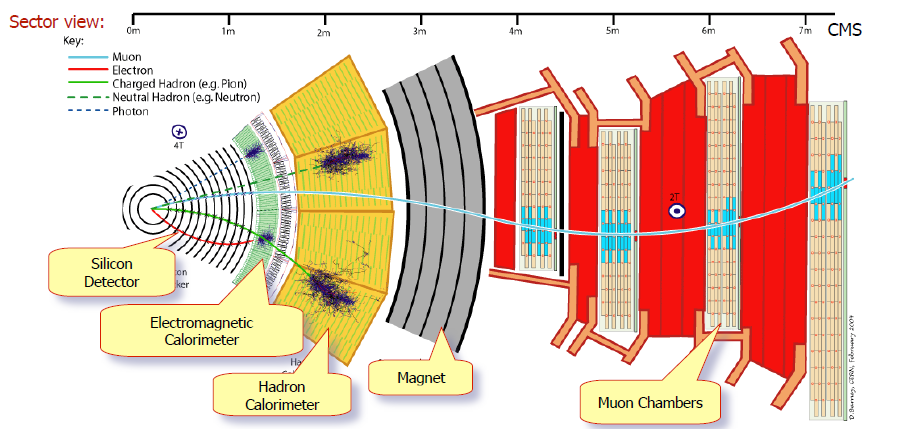
\includegraphics[scale=0.35]{Imag/reconstruccion_muones.png}
    \caption{Identificación de partículas en CMS, vista transversal del detector}
    \label{fig:my_label}
\end{figure}
    
\end{frame}

\begin{frame}{Definición de variables relevantes}

El detector CMS tiene una simetría cilindrica en donde el eje de colisi\'on es el "z" y el plano transversal esta formado por los ejes "x" e "y". Dos de las variables para caracterizar las propiedades de las partículas son las siguientes. 

    \begin{figure}[ht]
        \begin{minipage}[b]{0.45\linewidth}
            \centering
            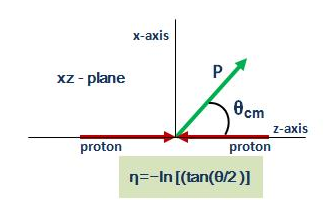
\includegraphics[width=\textwidth]{pseudorapidity.PNG}
            \caption{Definición de pseudorapidez}
            \label{fig:a}
        \end{minipage}
        \hspace{0.5cm}
        \begin{minipage}[b]{0.45\linewidth}
            \centering
            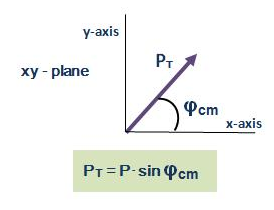
\includegraphics[width=\textwidth]{pt.PNG}
            \caption{Definición de momento transversal}
            \label{fig:b}
        \end{minipage}
    \end{figure}
    
\end{frame}

\begin{frame}{Parametrización de eficiencia y resolución}

Estas parametrizaci\'on est\'an contenidas en la simulaci\'on Delphes

%\color{red} Francisco aqui poner las graficas de eficiency y resolucion que habiamos obtenido examinando los datacards de Delphes, hacerlo para el detector actual (no HL-LHC)

    \begin{figure}[ht]
        \begin{minipage}[b]{0.45\linewidth}
            \centering
            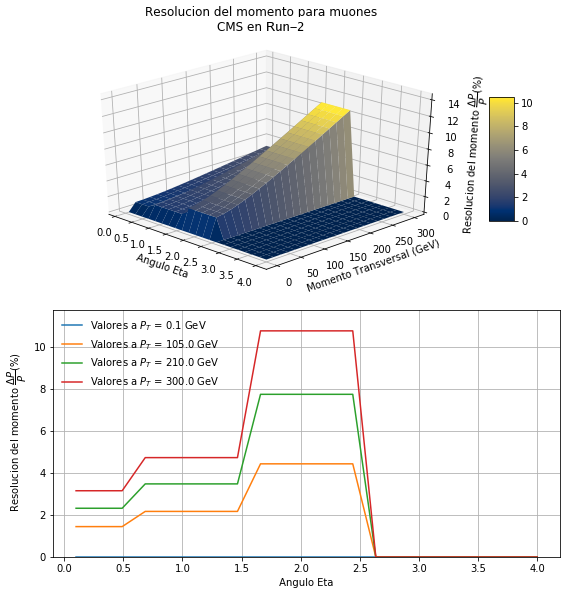
\includegraphics[width=\textwidth]{Imag/Momentum_resolution_of_Muon_CMS.png}
            \caption{Resolución del momento para muones.}
            \label{fig:a}
        \end{minipage}
        \hspace{0.5cm}
        \begin{minipage}[b]{0.45\linewidth}
            \centering
            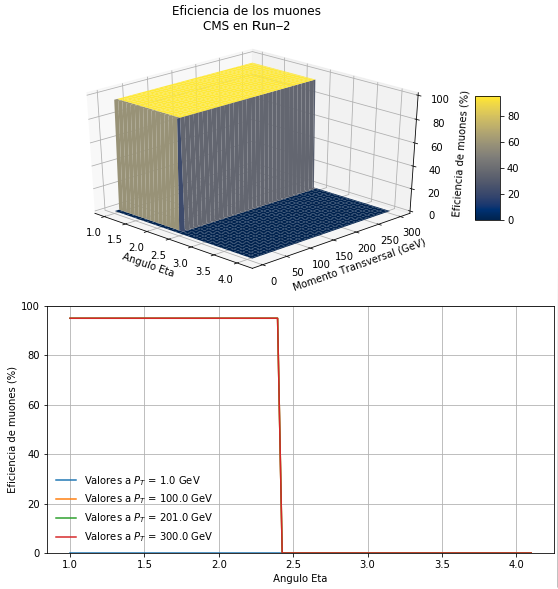
\includegraphics[width=\textwidth]{Imag/Eficiencia_of_Muon_CMS.png}
            \caption{Eficiencia en la reconstrucción de los muones.}
            \label{fig:b}
        \end{minipage}
    \end{figure}
    
\end{frame}

%\begin{frame}[fragile,allowframebreaks]{Herramientas de Caracterización}
\begin{figure}[h]
\centering
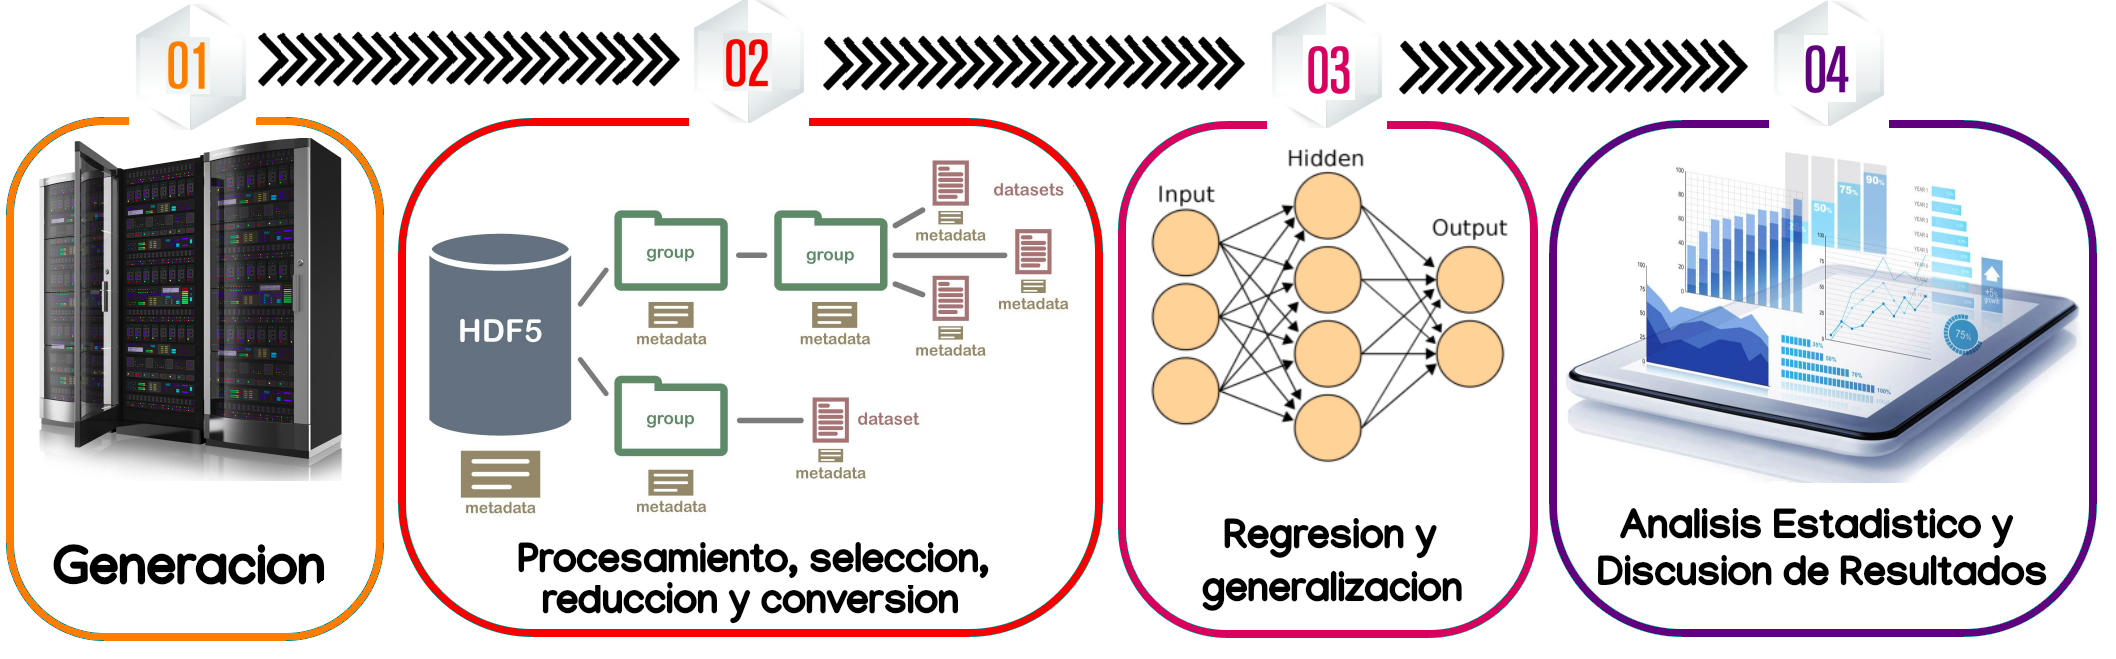
\includegraphics[width=1\textwidth]{Imag/procesos_darksusy.png}
\caption{Secuencia lógica de la investigación.}
\end{figure}

\framebreak

\begin{figure}[h]
\centering
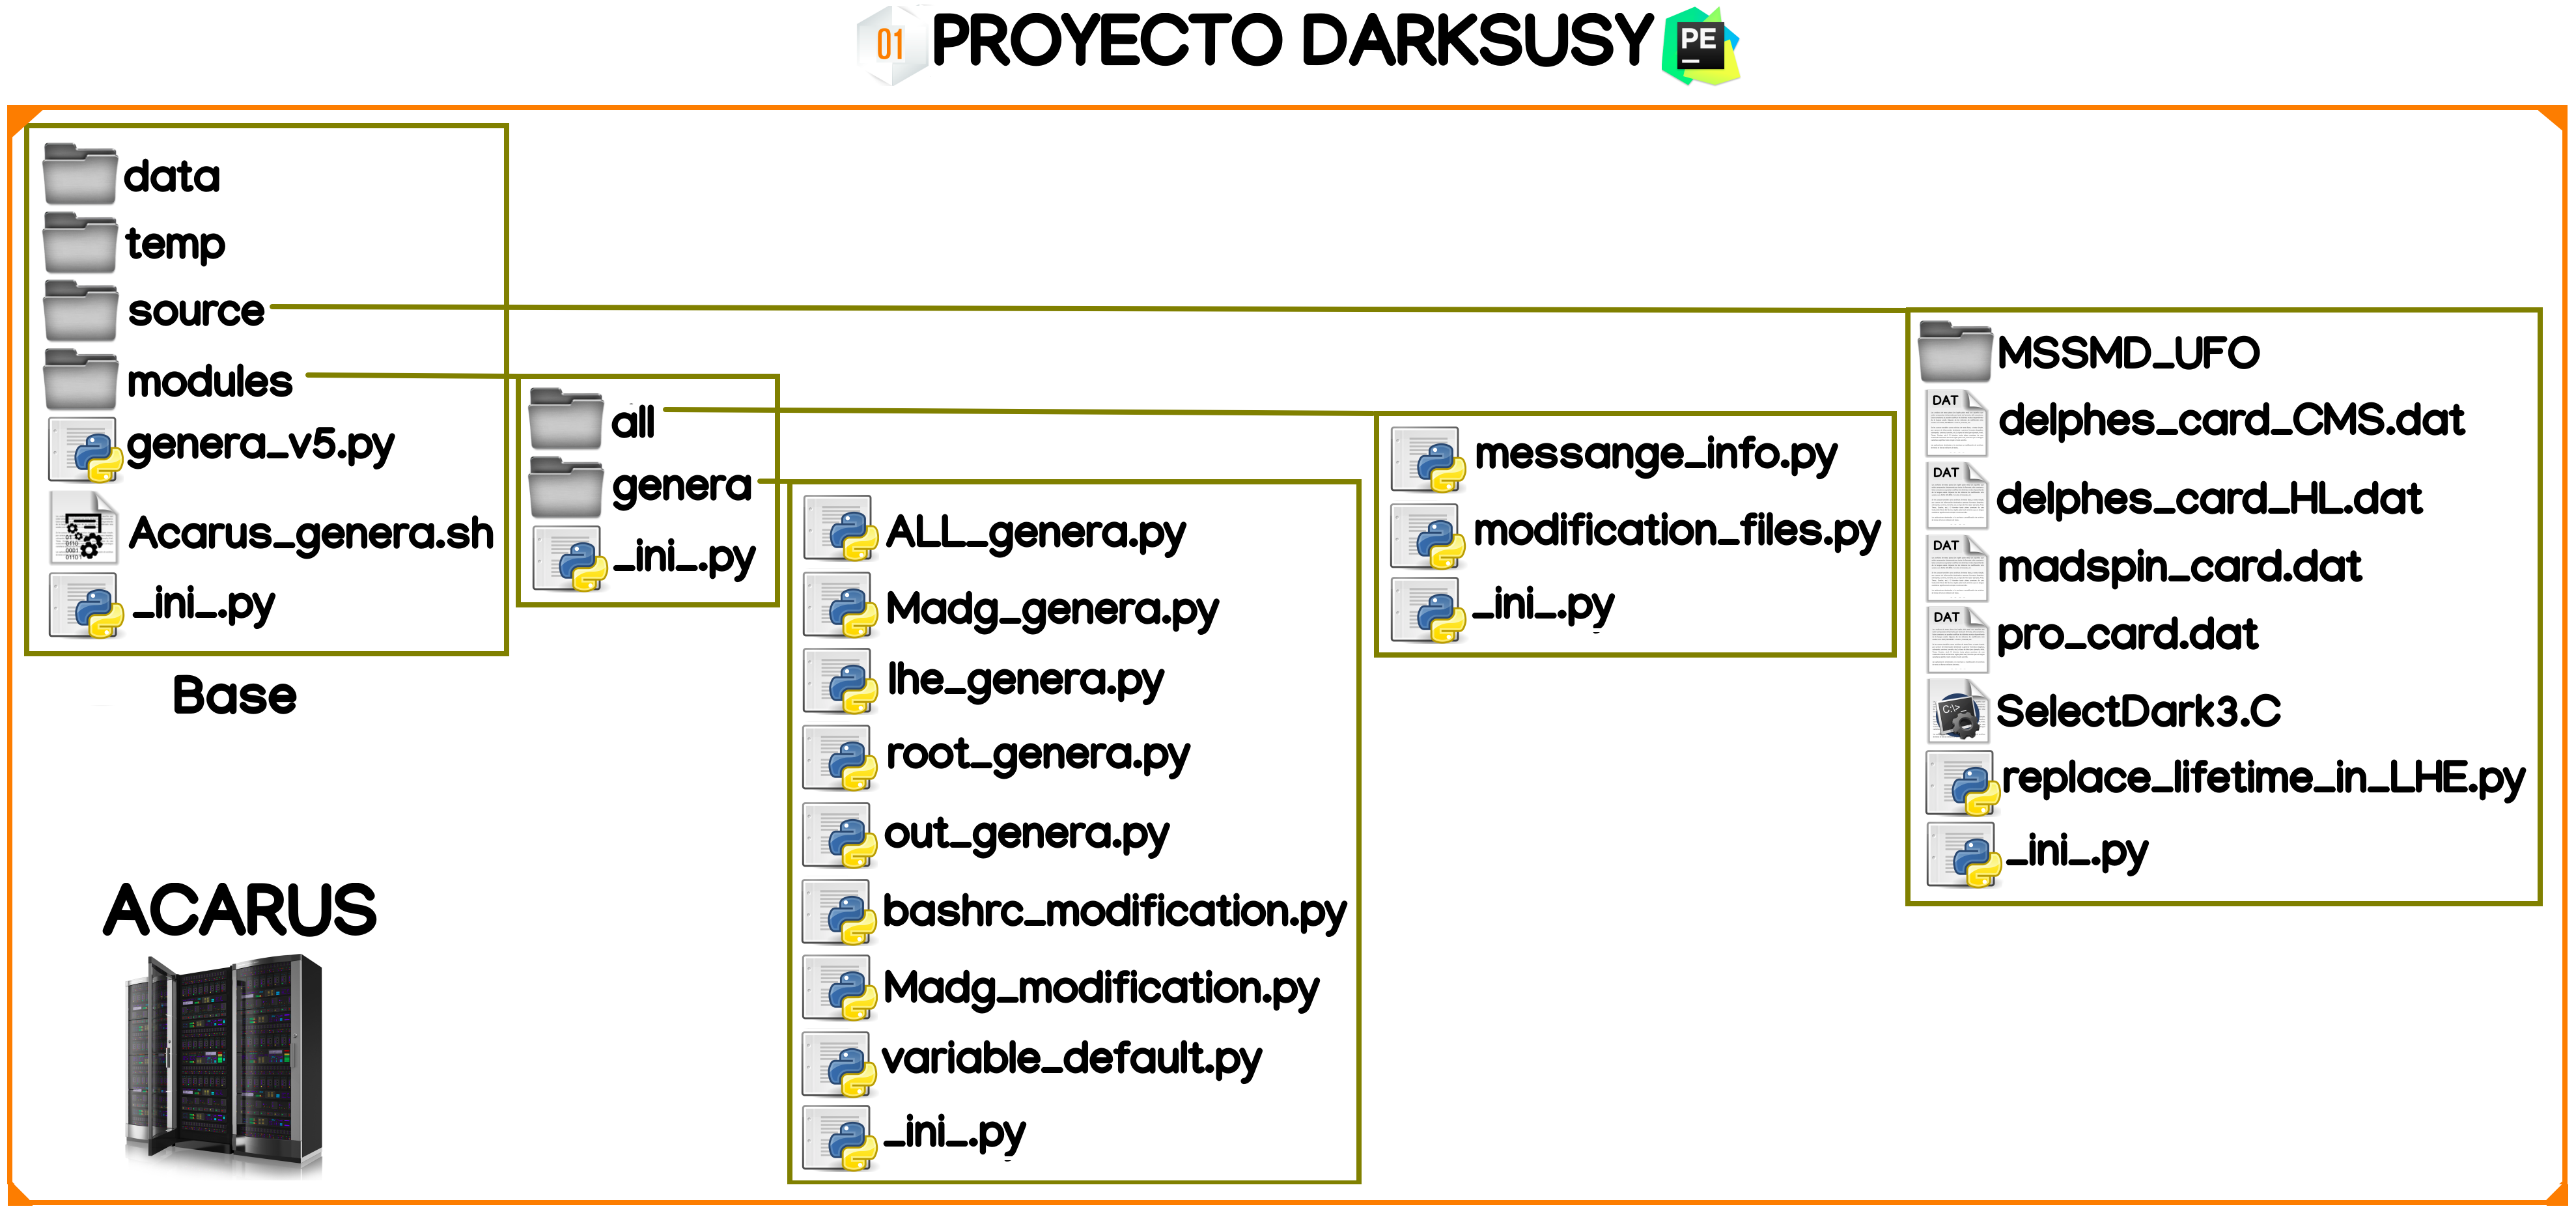
\includegraphics[width=1\textwidth]{Imag/proyecto_darksusy.png}
\caption{Estructura del proyecto generador.}
\end{figure}

\framebreak

\begin{figure}[h]
\centering
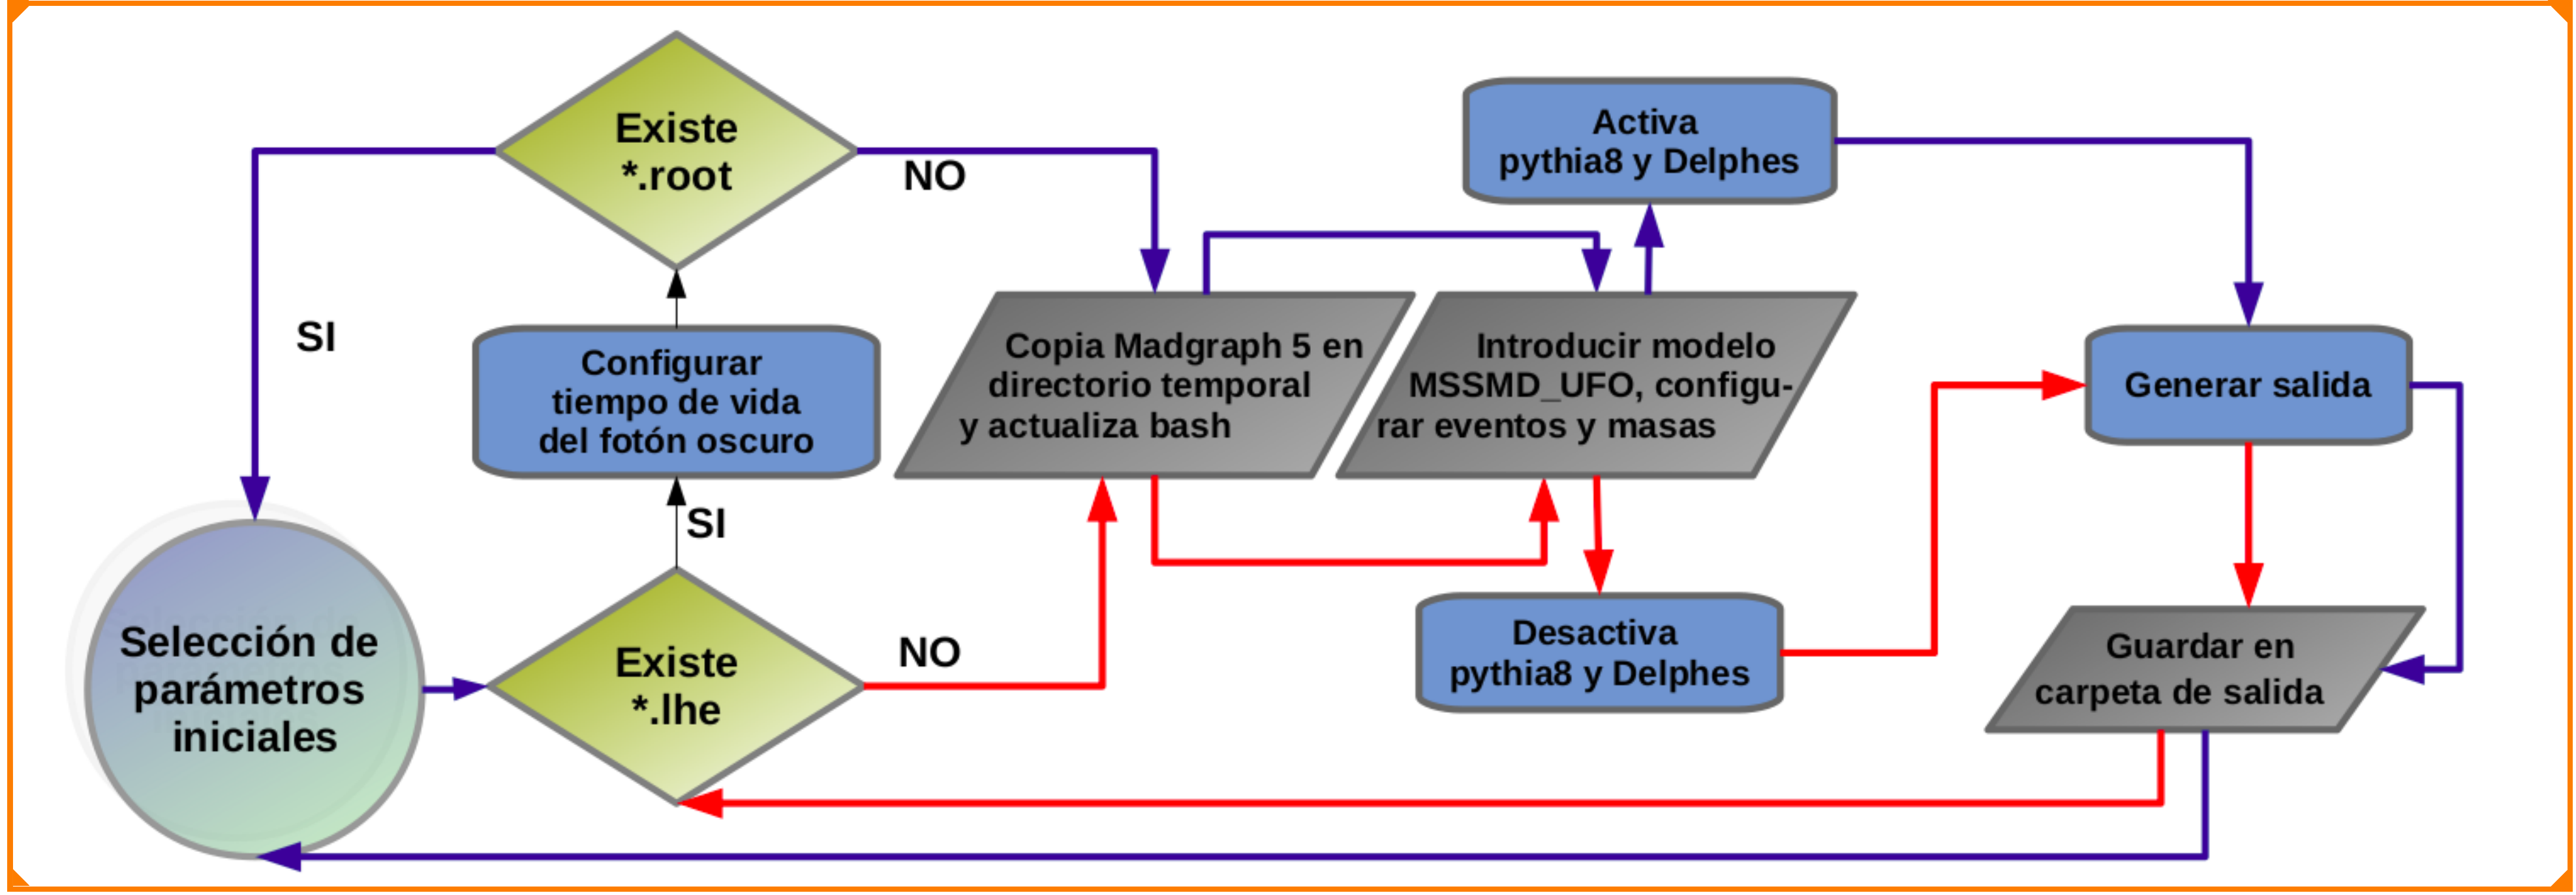
\includegraphics[width=1\textwidth]{Imag/proyecto_darksusy2.png}
\caption{Diagrama de Flujo del generador.}
\end{figure}

\framebreak

\begin{figure}[h]
\centering
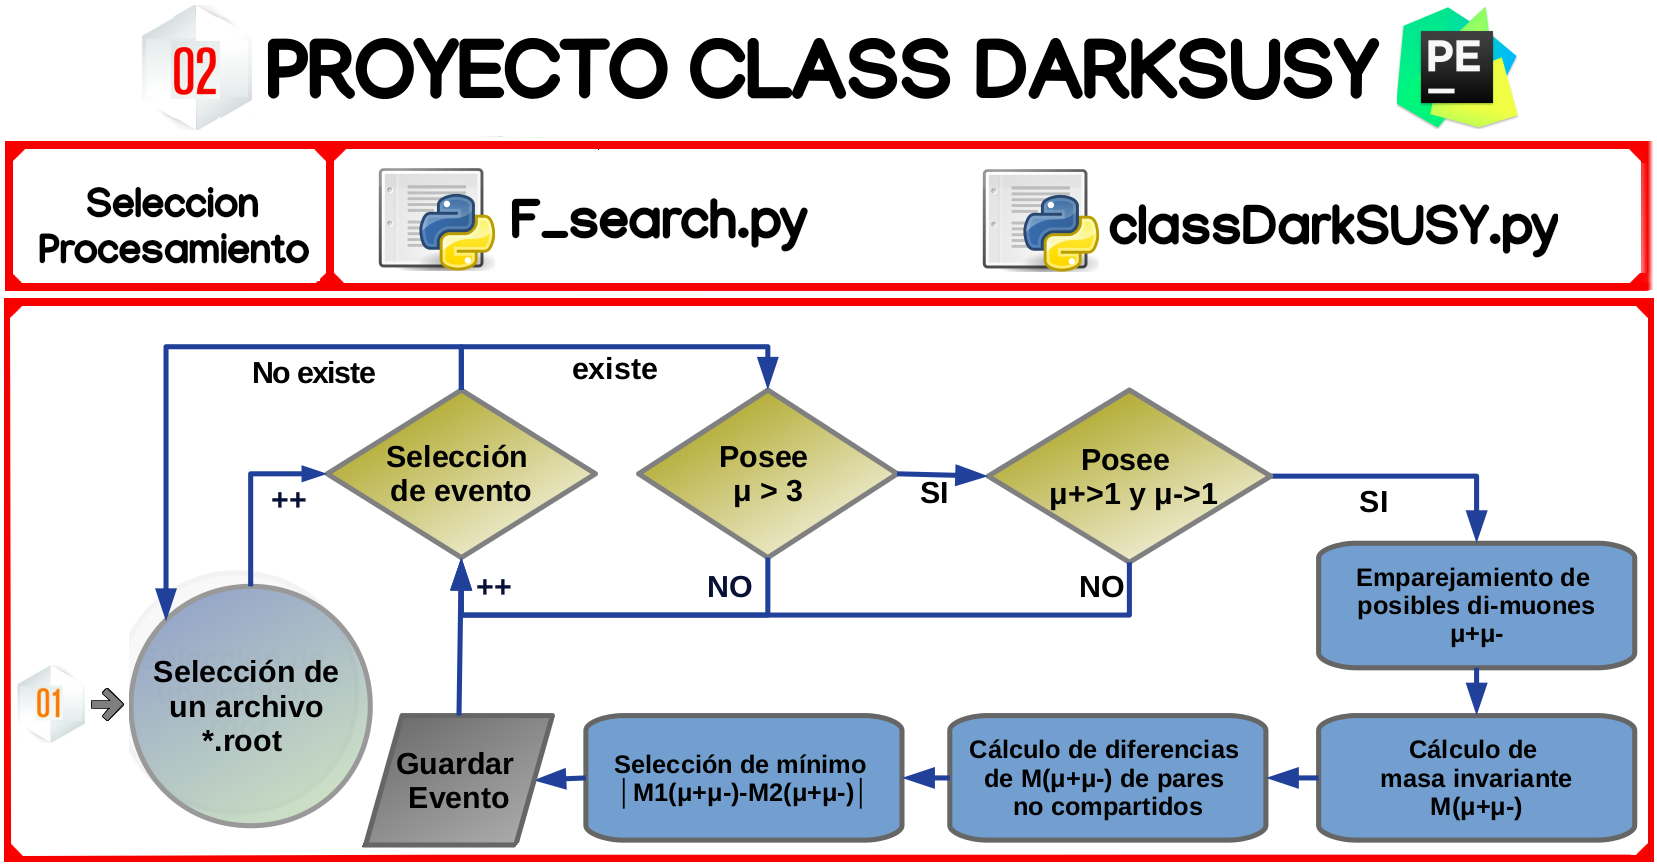
\includegraphics[width=1\textwidth]{Imag/class_darksusy.png}
\caption{Estructura del proyecto interpretador de la información $*.root$.}
\end{figure}

\framebreak

\begin{figure}[h]
\centering
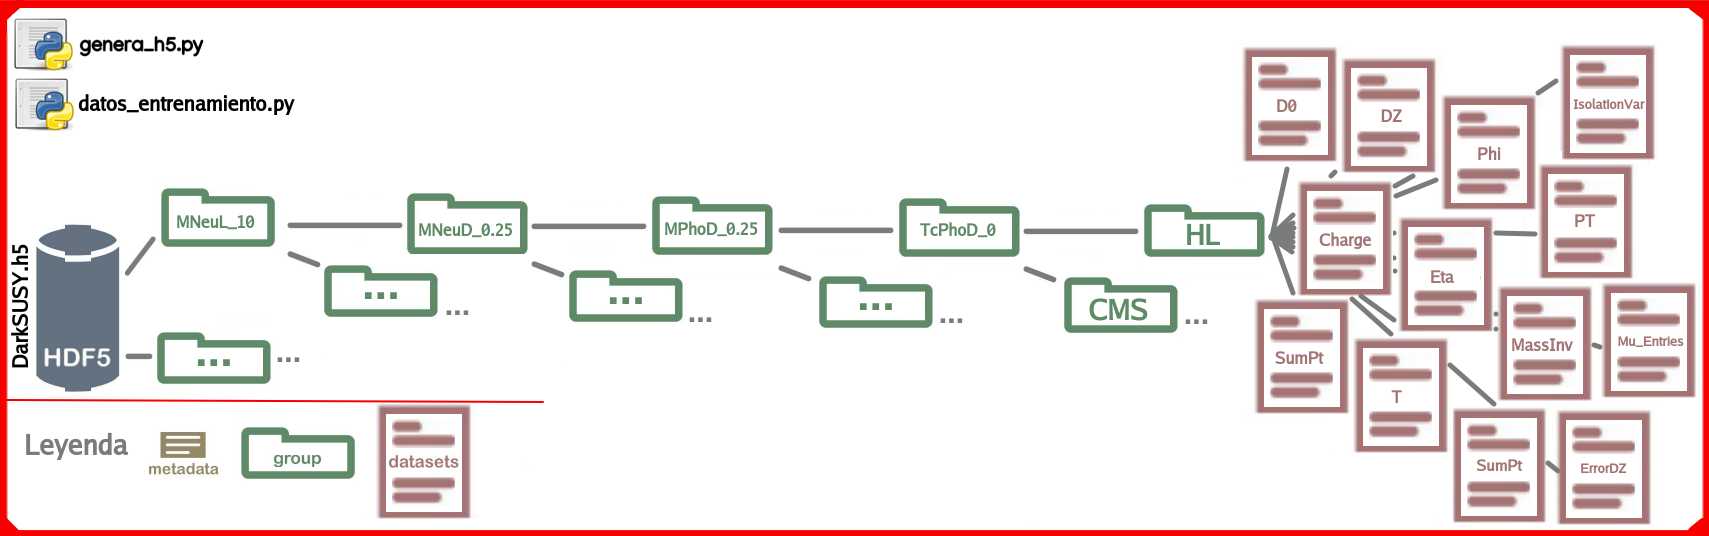
\includegraphics[width=1\textwidth]{Imag/class_darksusy3.png}
\caption{Estructura del archivo h5.}
\end{figure}
\end{frame}

\section{Análisis}
%\begin{frame}{}
    \begin{center}
        \LARGE Analisis
    \end{center}
\end{frame}


\begin{frame}{Estrategia del an\'alisis de datos}

\begin{itemize}
    \item El an\'alisis se basa en una selecci\'on de eventos a partir de una serie de variables experimentales las cuales buscan optimizar la eficiencia de la señal y reducir lo mas posible los procesos de ruido
    \item Recordar que en los datos experimentales solo se tiene informaci\'on de los muones reconstruidos y a partir de eso se infiere la posible producci\'on de fotones oscuros
    \item La selecci\'on de eventos se aplica a cada una de las muestras de simulaci\'on generadas y se estudia las eficiencias y distribuciones características 
\end{itemize}
    
\end{frame}


\begin{frame}{Secuencia del análisis de datos}

\begin{itemize}
    \item El análisis comienza con la muestra simulada (raw data) 
    \item Se procede a la selección de eventos, donde se reduce la cantidad de datos a analizar 
    \item Se procede a la obtención de resultados, gracias estadísticas y discusión de los mismos, algo similar al esquema mostrado en la figura 
\end{itemize}

\begin{figure}[h]
\centering
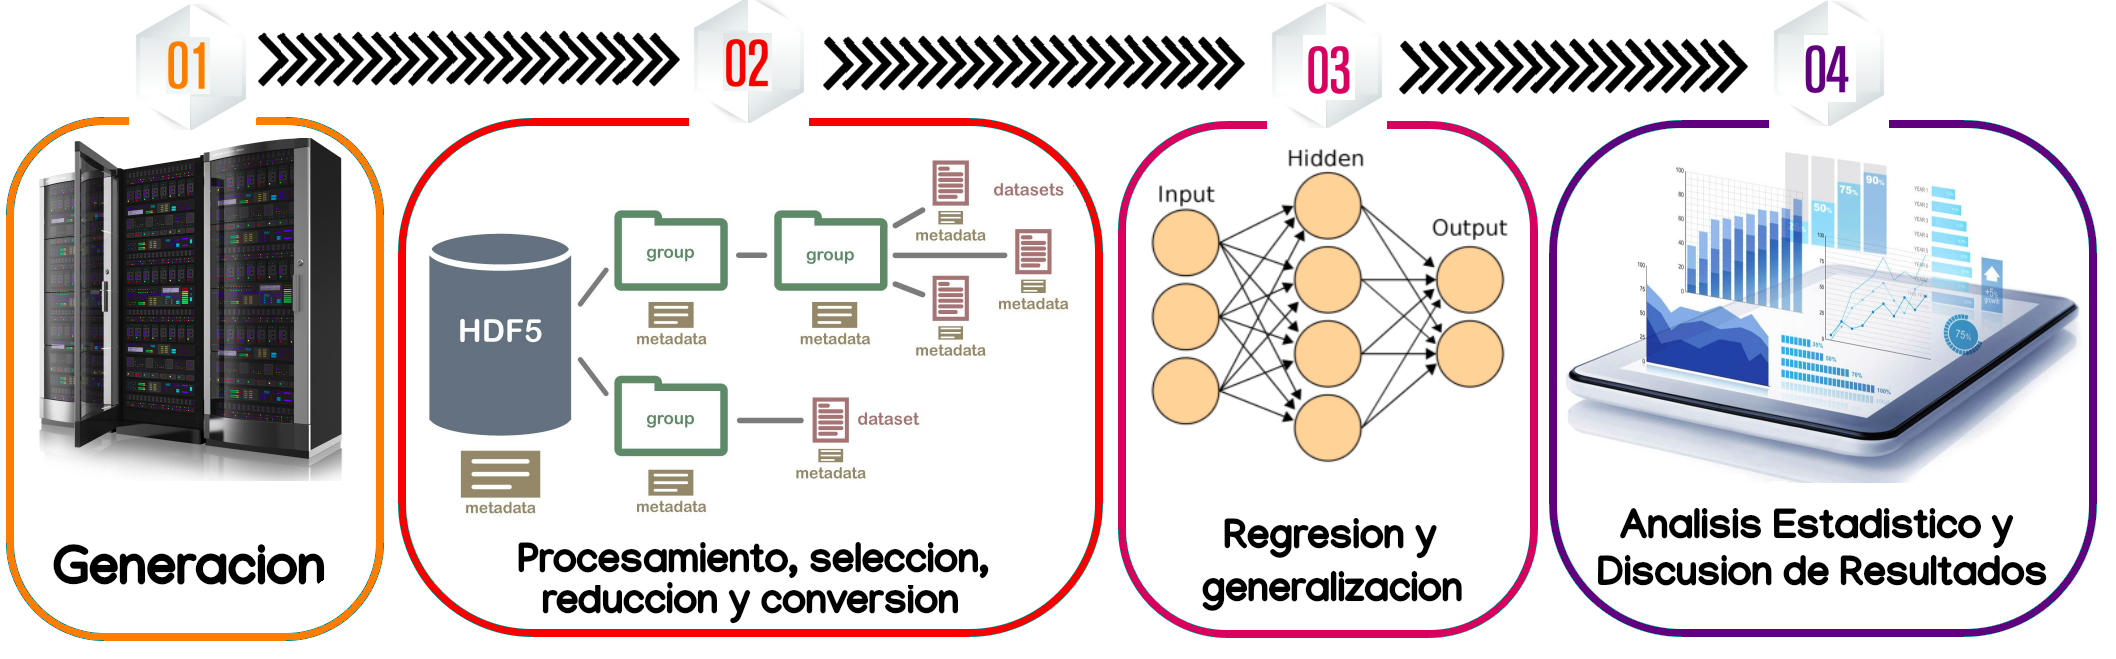
\includegraphics[width=0.8\textwidth]{Imag/procesos_darksusy.png}
\caption{Secuencia del análisis de datos}
\end{figure}

\end{frame}

\begin{frame}{Estructura del código de análisis}

\begin{itemize}
    \item Se desarrollo un entorno de simulaci\'on y an\'alisis de datos el cual esta basado en código de python y ROOT. 
    \item El entorno se encuentra hospedado en ACARUS y puede ser fácilmente extendido para el análisis de otros modelos (adicionales a Dark-SUSY)
\end{itemize}
    
\begin{figure}[h]
\centering
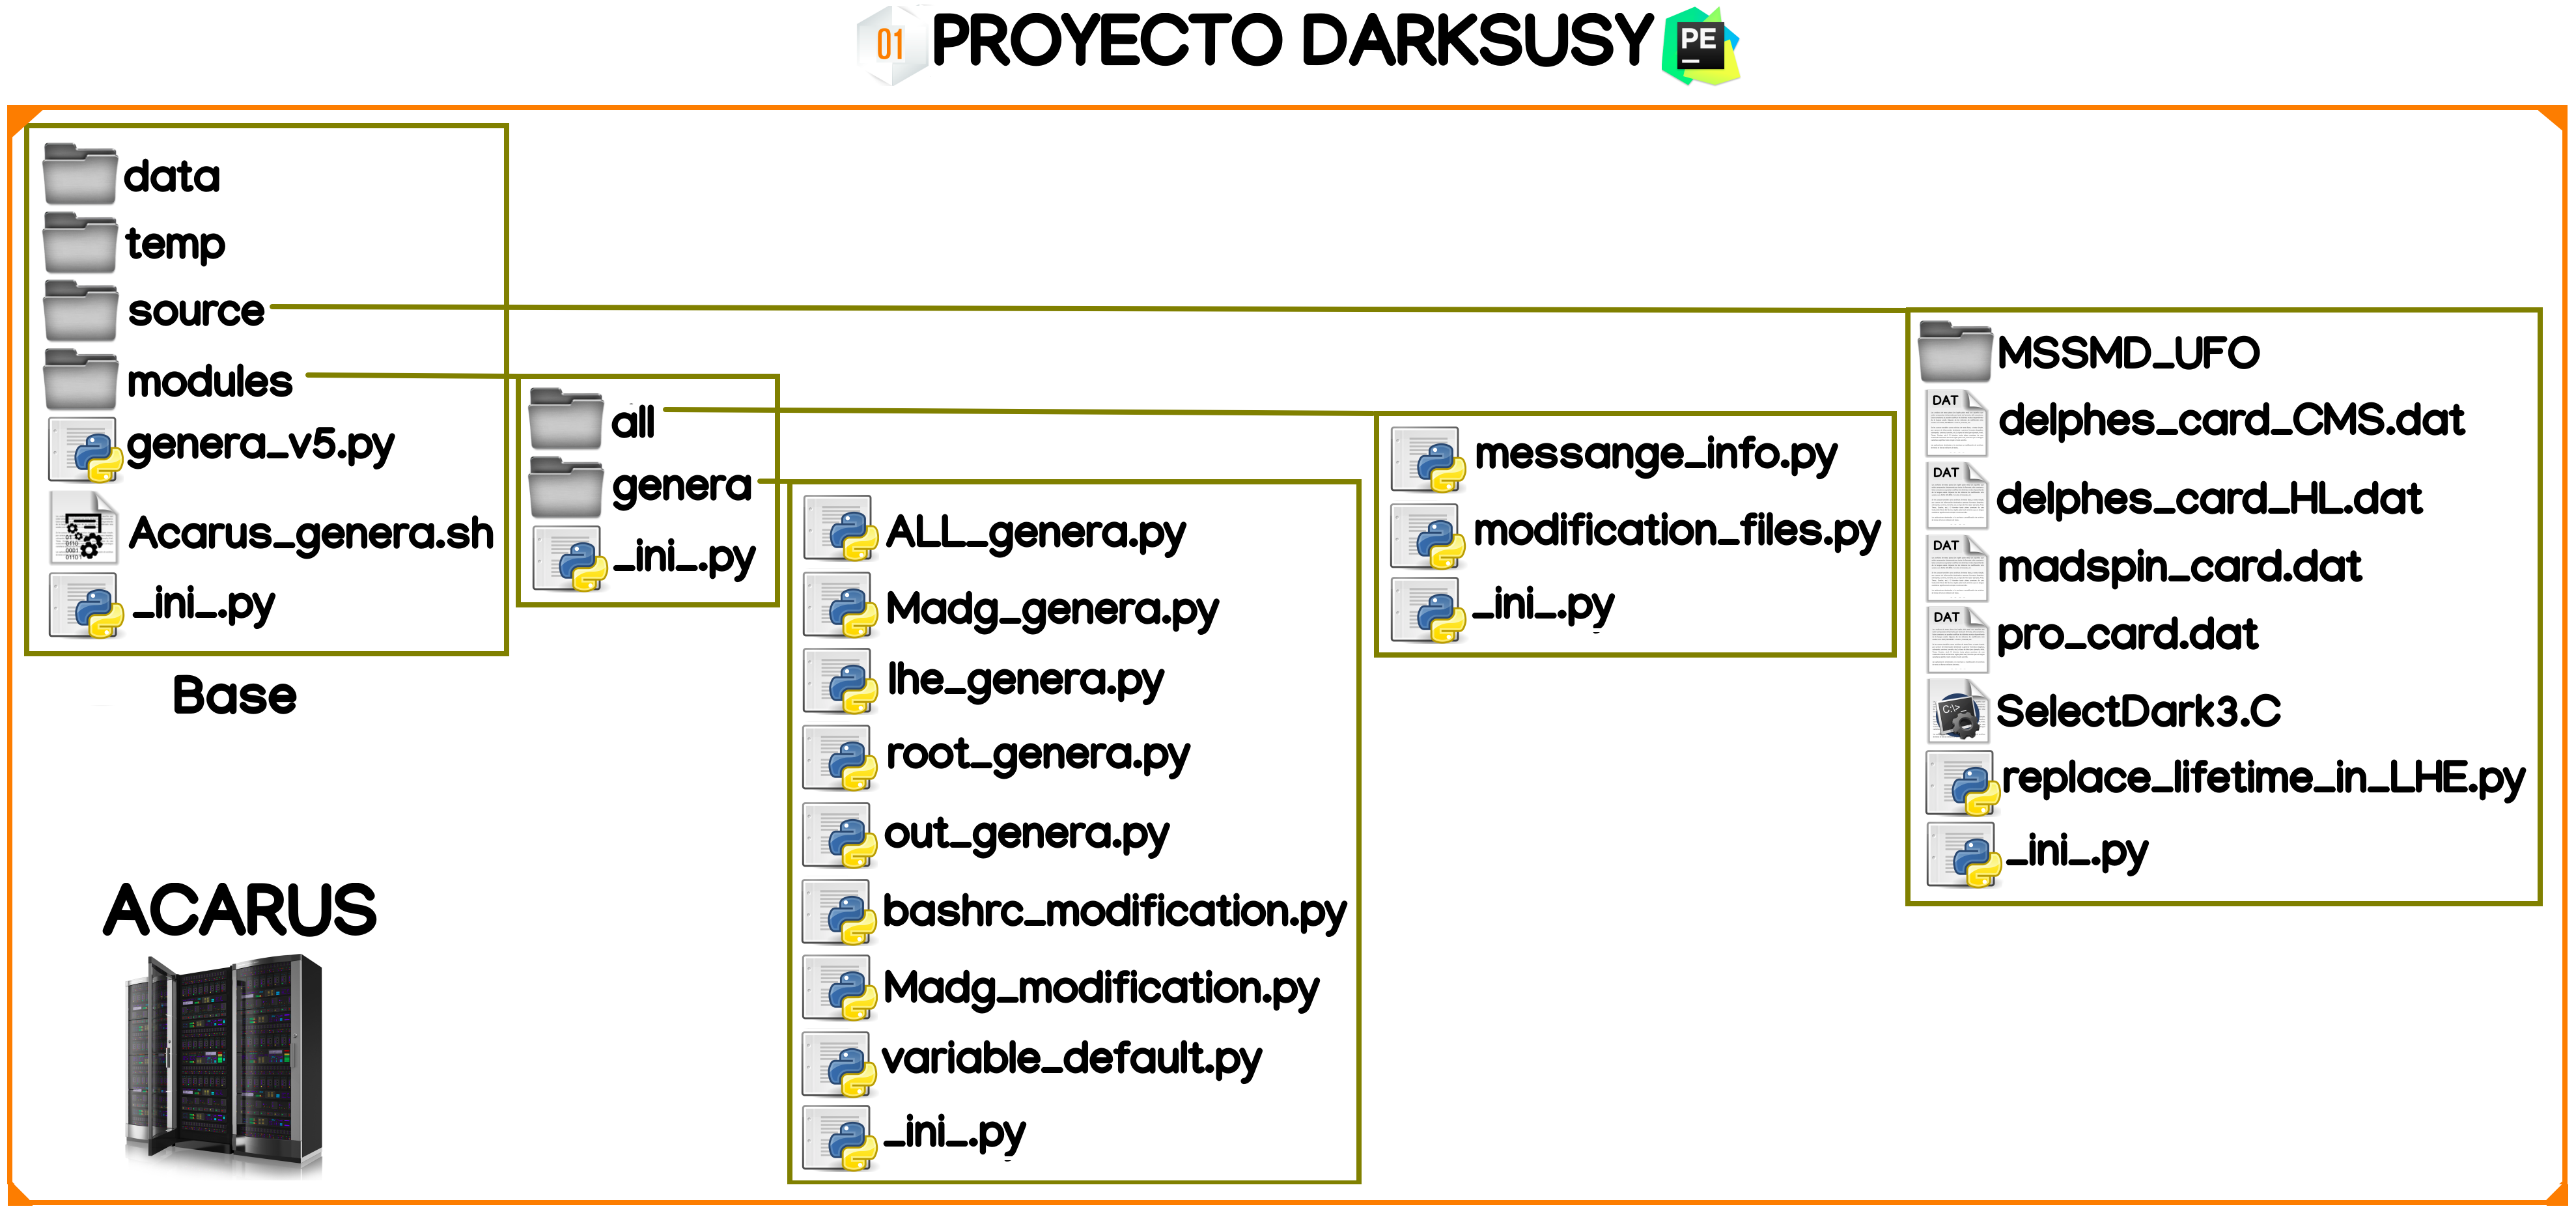
\includegraphics[width=0.8\textwidth]{Imag/proyecto_darksusy.png}
\caption{Estructura del código de análisis}
\end{figure}

\end{frame}



\begin{frame}{Selección preliminar}

\begin{itemize}
    \item \textbf{4$\mu$}: Selecci\'on de eventos con al menos 4 muones
    \begin{itemize}
        \item Muones con un momento transversal ($p_{T}$) mayor a
        \item Muones con un valor de pseudo-rapidez ($|\eta|$) menor a 2.4
    \end{itemize}
    \item \textbf{Algoritmo de pariamiento de muones}: Encontrar el par de muones optimos que con mayor probabilidad podrian ser generados por un foton oscuro
\end{itemize}
    
\end{frame}


\begin{frame}{Algoritmo de pariamiento de muones}
%\color{red} Francisco aqui incluir el diagrama de algoritmo de pariamiento
\begin{figure}[h]
\centering
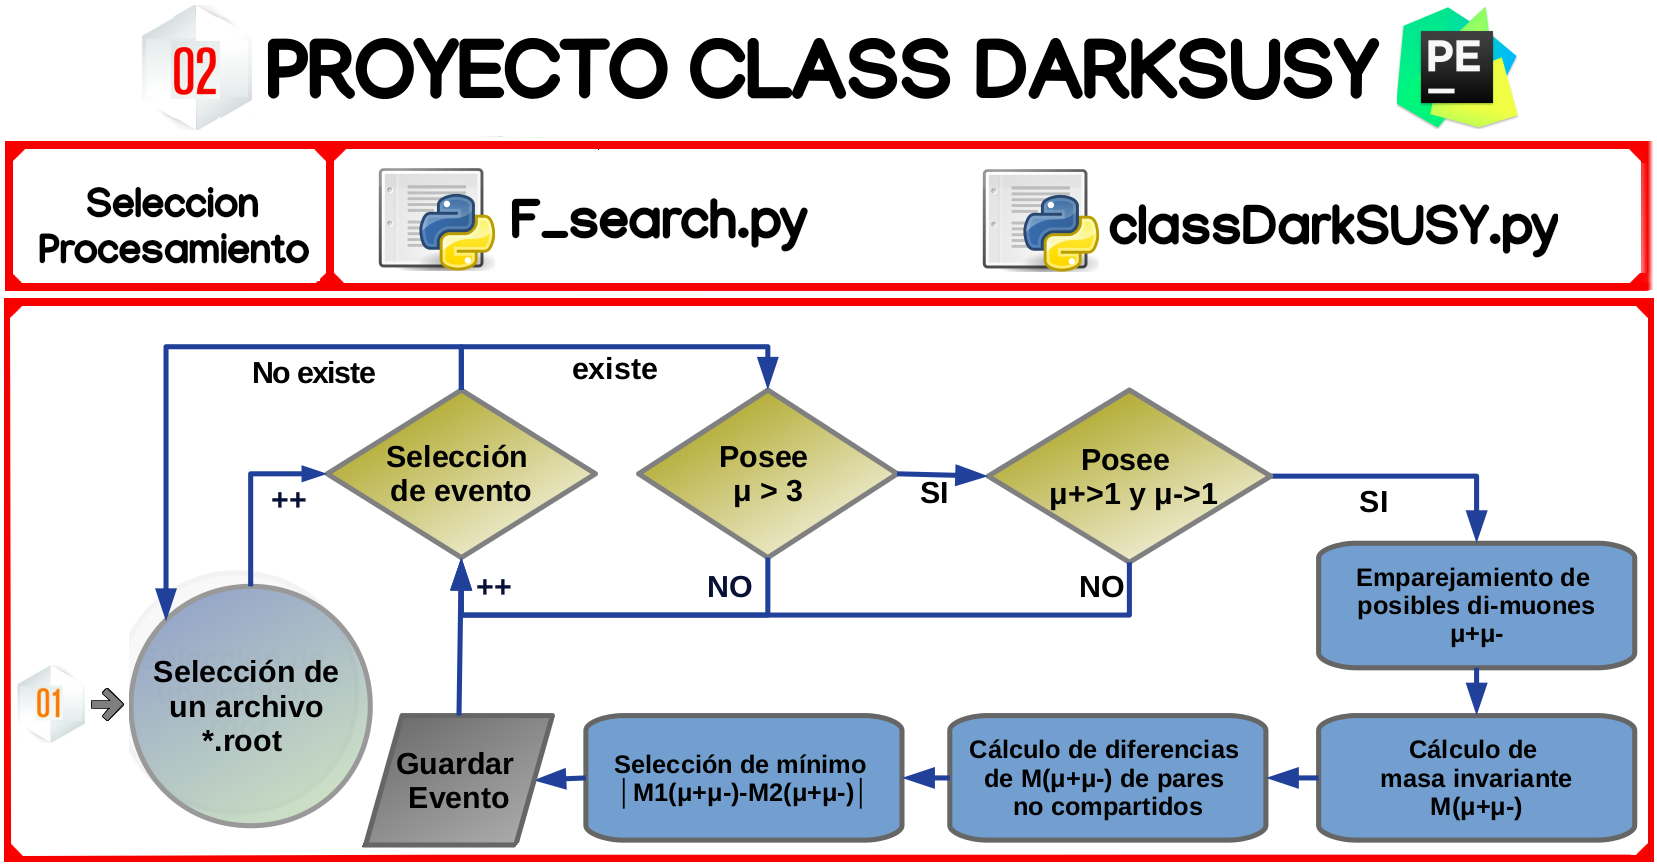
\includegraphics[width=1\textwidth]{Imag/class_darksusy.png}
\caption{Diagrama de algoritmo de pariamiento.}
\end{figure}   
\end{frame}

\begin{frame}{Eficiencia para fot\'on oscuro de baja masa}
\color{red} Francisco llenar estos numeros \color{black}
\begin{table}[]
    \centering
    \begin{tabular}{c|c|c|c|c|c|}
Selecci\'on  & $c\tau=XX$ & $c\tau=XX$ & $c\tau=XX$ & $c\tau=XX$ & $c\tau=XX$ \\  \hline
Sin corte         &  XXX & XXXX & XXXX & XXXX & XXX \\
4-$\mu$         &  XXX & XXXX & XXXX & XXXX & XXX \\
pariamiento    &  XXX & XXXX & XXXX & XXXX & XXX
     \end{tabular}
    \caption{Tabla con el numero de eventos despu\'es de cada selecci\'on $m_{\gamma_{D}}$=0.25 y diferentes valores del tiempo de vida}
    \label{tab:my_label}
\end{table}
    
\end{frame}

\begin{frame}{Eficiencias fot\'on oscuro de altas masa}
\color{red} Francisco llenar estos numeros \color{black}

\begin{table}[]
    \centering
    \begin{tabular}{c|c|c|c|c|c|}
Selecci\'on  & $c\tau=XX$ & $c\tau=XX$ & $c\tau=XX$ & $c\tau=XX$ & $c\tau=XX$ \\ \hline
Sin corte         &  XXX & XXXX & XXXX & XXXX & XXX \\
4-$\mu$         &  XXX & XXXX & XXXX & XXXX & XXX \\
pariamiento    &  XXX & XXXX & XXXX & XXXX & XXX
     \end{tabular}
    \caption{Tabla con el numero de eventos despu\'es de cada selecci\'on $m_{\gamma_{D}}$= 8~\GeV y diferentes valores del tiempo de vida}
    \label{tab:my_label}
\end{table}
    
\end{frame}


\begin{frame}{Distribuciones características: Masa invariante}
    
    \begin{itemize}
        \item Después de la selección preliminar se puede reconstruir la masa de los muones, dicha masa correspondería a la masa de los fotones oscuros. A continuación se muestra un ejemplo para los procesos con un valor esperado de $m_\gamma = 4 GeV$ :%\color{red} Francisco incluir estos gráficos 
    \end{itemize}
    
    \begin{figure}[ht]
    \centering
    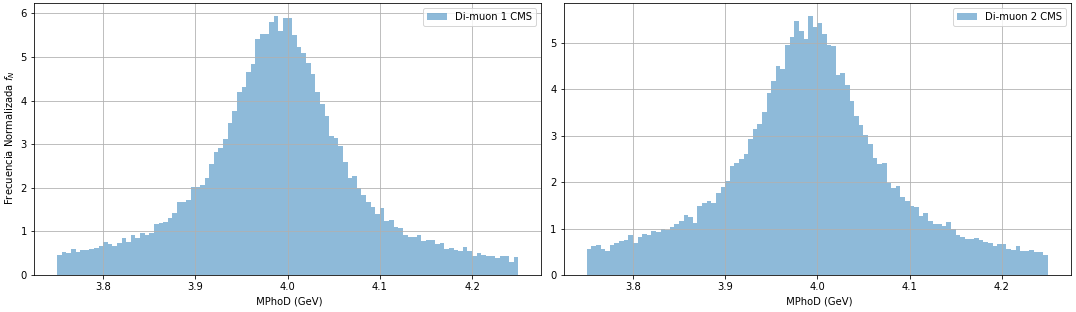
\includegraphics[width=1\textwidth]{Imag/Datos_Photon4muon_CORTE_CMS.png}
    \caption{Masa invariante para los di-muones.}
    \end{figure}
%    \begin{figure}[ht]
%        \begin{minipage}[b]{0.45\linewidth}
%            \centering
%            
\includegraphics[width=\textwidth]{placeholder.png}
%            \caption{Masa invariante primer di-muon}
%            \label{fig:a}
%        \end{minipage}
%        \hspace{0.5cm}
%        \begin{minipage}[b]{0.45\linewidth}
%            \centering
%            
\includegraphics[width=\textwidth]{placeholder.png}
%            \caption{Masa invariantes segundo di-muon}
%            \label{fig:b}
%        \end{minipage}
%    \end{figure}
\end{frame}

\begin{frame}{Distribuciones caracteristicas: Parametro de impacto (d0)}
    \color{red} Francisco incluir estos graficos (para el detector actual, todaviano no HL-LHC)
\end{frame}

\begin{frame}{}
    \begin{center}
        \LARGE High Luminosity LHC
    \end{center}
\end{frame}

\begin{frame}{Etapa de Alta luminosidad para el Gran Colisionador de Hadrones}
    \begin{itemize}
        \item El Gran Colisionador de Hadrones junto con sus experimentos principales estan en una etapa de actualizacion en preparacion para la etapa de alta luminosidad (2025-2035) 
        \item En particular para la deteccion de muones se instalaran una serie de nuevos detectores que ampliaran el rango de deteccion, muy en particular para la region de pseudo-rapidez ($2.4<|\eta|<3.0$) como se muestra en el la imagen
        \item Estos nuevos detectores permitiran la identificacion de muones en esta region, y aumentaran la probabilidad de detectar se\~nales como los fotones oscuros
    \end{itemize}
\end{frame}

\begin{frame}{Acutalizaci\'on del sistema de muones en el HL-LHC}

\begin{itemize}
    \item La actualizaci\'on de basa en la instalaci\'on de nuevos detectores de muones 
    \item Dicha detecci\'on amplia el rango de b\'usqueda para la posible detecci\'on de muones provenientes del fot\'on oscuro y otros modelos de fisica mas alla del modelo est\'andar
\end{itemize}

\begin{figure}
    \centering
    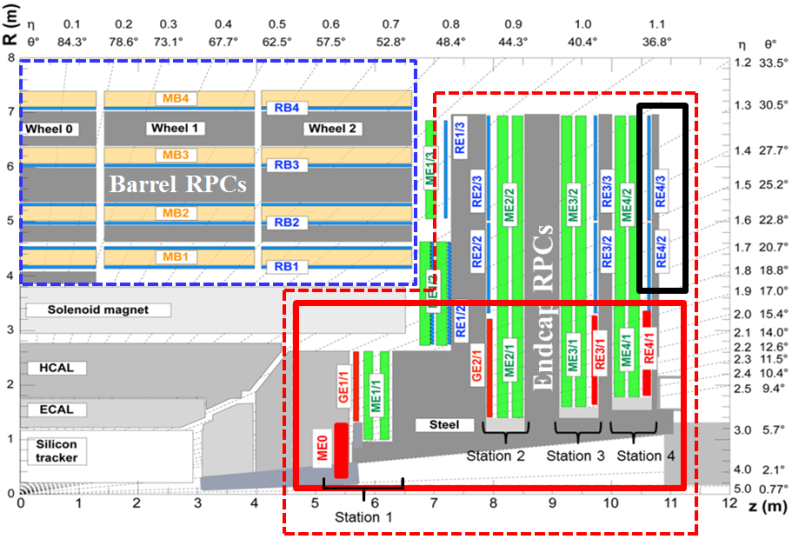
\includegraphics[width=1\textwidth]{muon_phase-2.png}
    \caption{Actualizacion del sistema de muones para la fase de alta luminosidad}
    \label{fig:my_label}
\end{figure}
    
\end{frame}


\begin{frame}{Comparacion distribuciones detector actual vs HL-LHC}
%\color{red} Francisco aqui poner distribucion de pseudorapidez comparando el detector actual y el detector nuevo
\begin{figure}
    \centering
    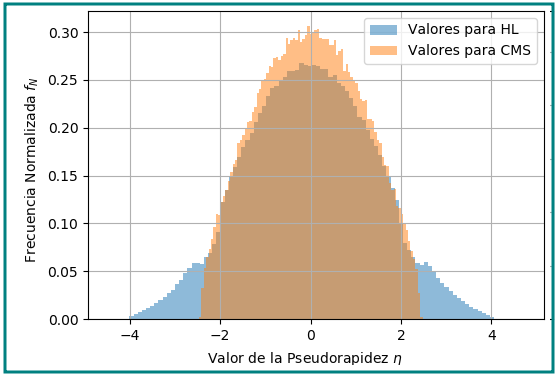
\includegraphics[width=1\textwidth]{Imag/Datos_Eta_ALL_simple.png}
    \caption{Comparar pseudorapidez.}
    \label{fig:my_label}
\end{figure}  
\end{frame}

\begin{frame}{Comparación de eficiencias detector actual vs HL-LHC.}
    
    \begin{itemize}
        \item Las ventajas de las actualizaciones se ve reflejada como una aumento en la eficiencia de la se\~nal
        \item La b\'usqueda del fot\'on oscuro durante el HL-LHC es uno de los objetivos fundamentales
    \end{itemize}
    
\begin{figure}[h]
\centering
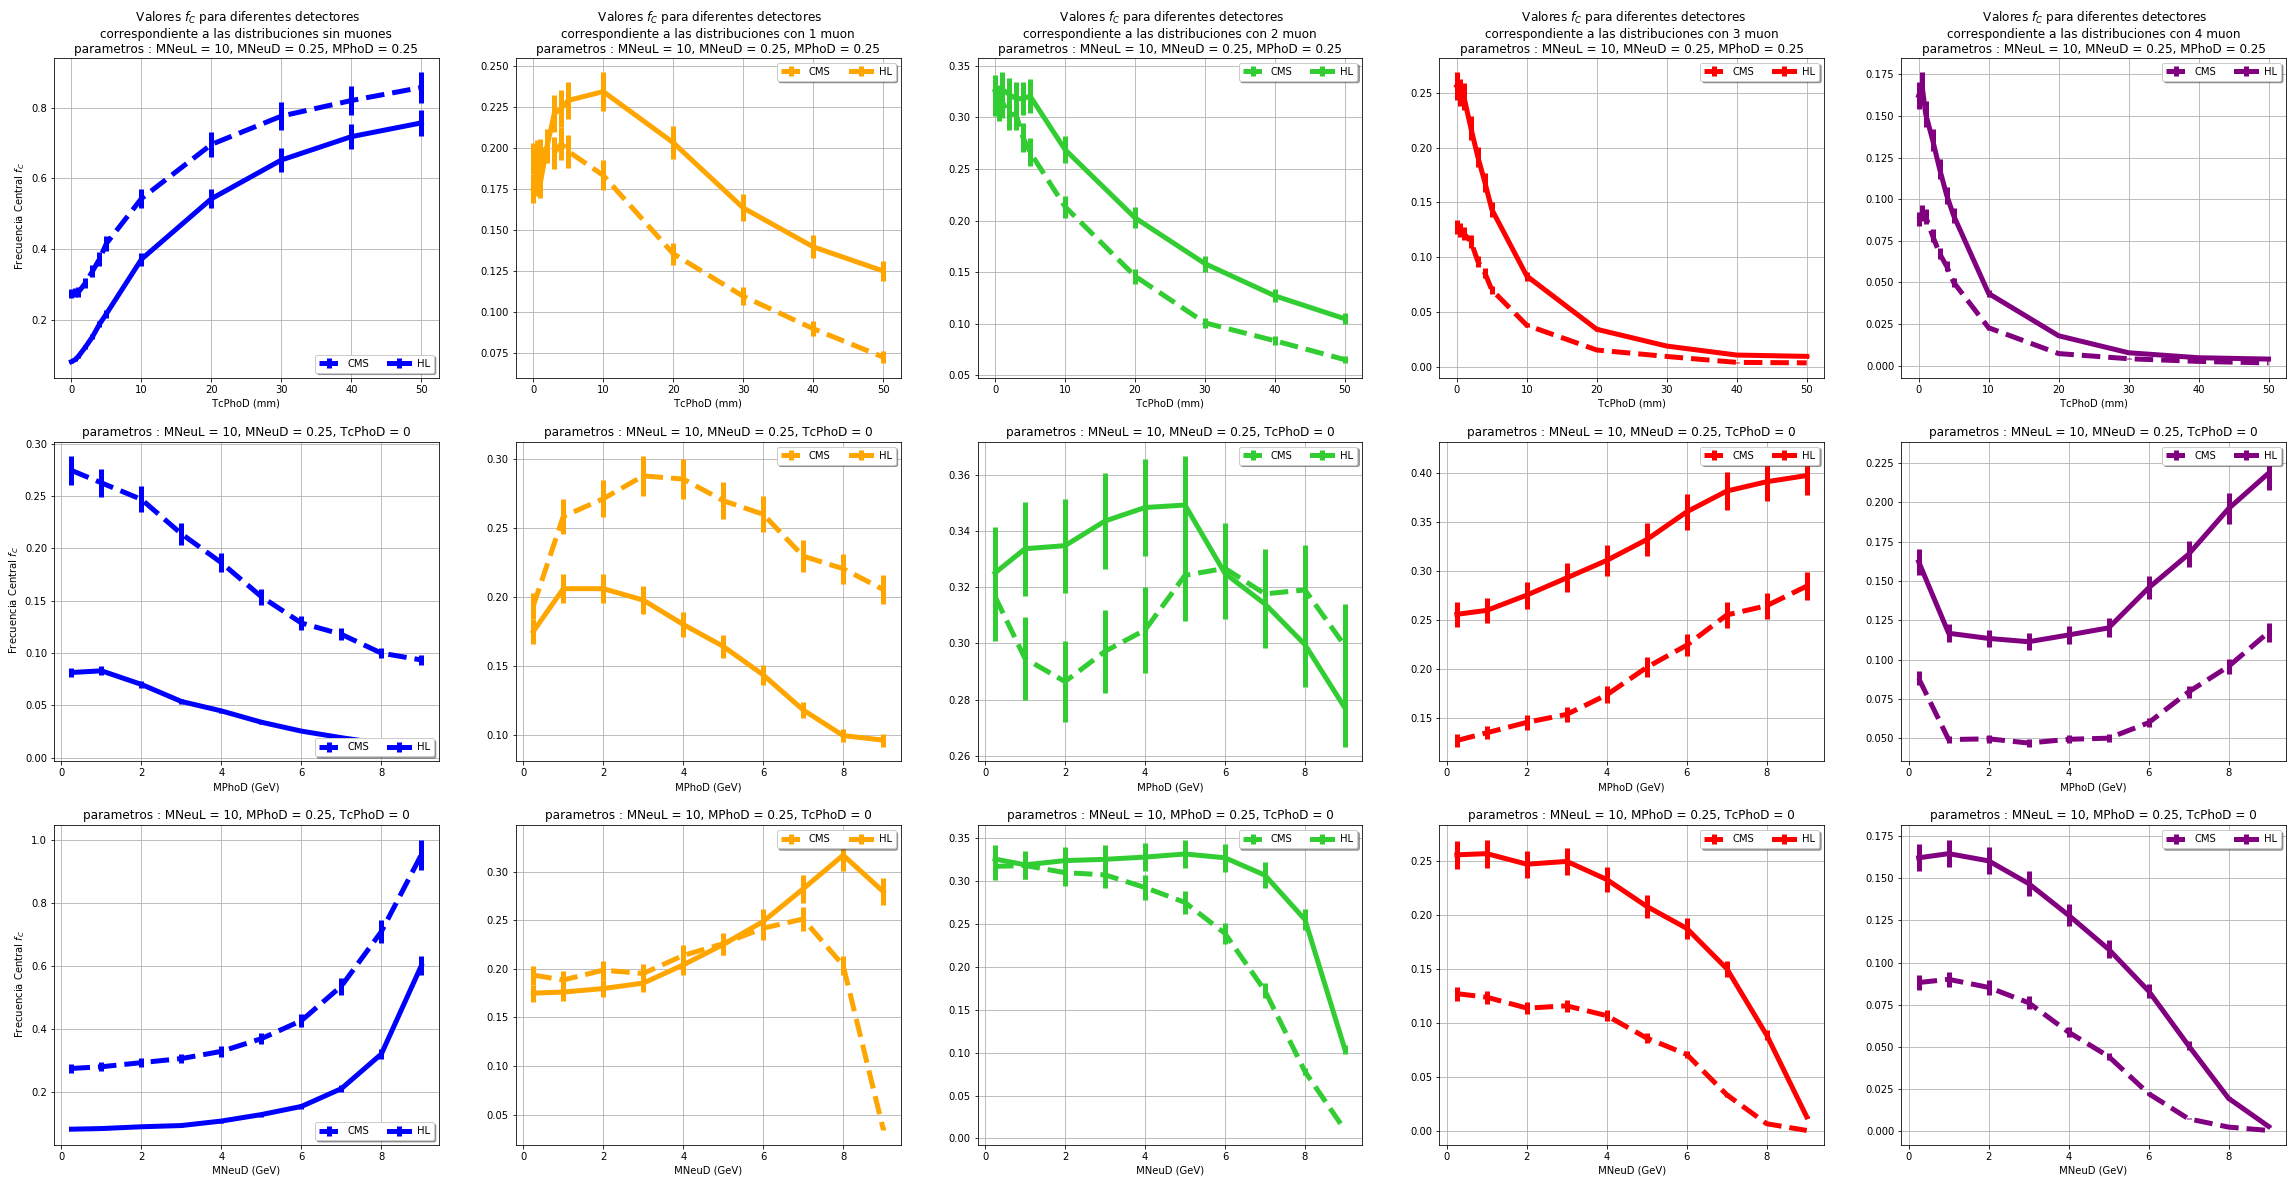
\includegraphics[width=0.8\textwidth]{Imag/Comparacion_Distribucion_Entries.png}
\caption{Comparacion de eficiencias del detector actual vs HL-LHC para las diferentes muestras}
\end{figure}

\end{frame}

\begin{frame}{Resumen}
\begin{itemize}
    \item Se integro el modelo Dark-SUSY en un entorno de simulacion
    \item Se desarrollo un entorno de simulaci\'on y an\'alisis el cual usa los recursos computacionales de la Universidad de Sonora (ACARUS) para generar resultados 
    \item Se estudio a detalle la se\~nal caracteristica de los fotones oscuros
    \item Se comparo la mejora en cuanto a eficiencia y rango de busqueda en la reconstruccion de muones del detector actual respecto a la actualizaci\'on en la etapa de alta luminosidad (HL-LHC) concluyendo que se tendra en general una mejor de \color{red} Francisco poner una estimacion de este numero XXX\% \color{black} de eficiencia en la b\'usqueda de esta se\~nal
\end{itemize}
    
\end{frame}


\begin{frame}{Siguientes Pasos}
\begin{itemize}
    \item Finalizar escritura de tesis (Finales de Junio) 
    \item Distribuir primer draft a  principios de Julio
    \tiem Presentar a finales de Julio o principios de Agosto
\end{itemize}
    
\end{frame}


%\begin{frame}{}
    \begin{center}
        \LARGE Backup
    \end{center}
\end{frame}
    


\begin{frame}{Estrategia de Simulacion}
El elemento iniciador se encuentra en la función \texttt{genera\_v5.py} versión 5, con este se incluye una descripción de opciones que hacen que sea adaptable ante situaciones alternativas a su configuración original:\\
\begin{scriptsize}
\texttt{
\begin{tabular}{ll}
genera\_v5.py [-h] & [-Event EVENT] [-MNeuD MNEUD] [-MNeuD MNEUD]\\
& [-MPhoD MPHOD] [-TcPhoD TCPHOD] [-Mode MODE]\\
& [-Card CARD] [-Name NAME] [-Dir\_Madg DIR\_MADG]\\
& [-Dir\_temp\_Madg DIR\_TEMP\_MADG] [-Dir\_Source DIR\_SOURCE]\\
& [-Dir\_Out DIR\_OUT]\\
\end{tabular}}
\end{scriptsize}
\begin{tiny}
\texttt{
\begin{tabular}{ll}
optional arguments:&\\
-h, --help & Show this help message and exit\\
-Event EVENT & Number of Event\\
-MNeuD MNEUD & Mass of the Dark Neutralino\\
-MNeuL MNEUL & Mass of the Lightest Neutalino\\
-MPhoD MPHOD & Mass of the Dark Photon\\
-TcPhoD TCPHOD & Life time of the Dark Photon\\
-Mode MODE & Condition using ``in'' or ``out''\\
-Card CARD & Card using ``CMS'' or ``HL''\\
-Name NAME & Name of root file out\\
-Dir\_Madg DIR\_MADG & Directory of Madgraph\\
-Dir\_temp\_Madg DIR\_TEMP\_MADG & Directory of temporal install Madgraph\\
-Dir\_Source DIR\_SOURCE & Directory where source stay\\
-Dir\_Out DIR\_OUT & Directory of result\\
\end{tabular}}
\end{tiny}
\end{frame}

\begin{frame}[fragile,allowframebreaks]{Herramientas de Caracterización}
\begin{figure}[h]
\centering
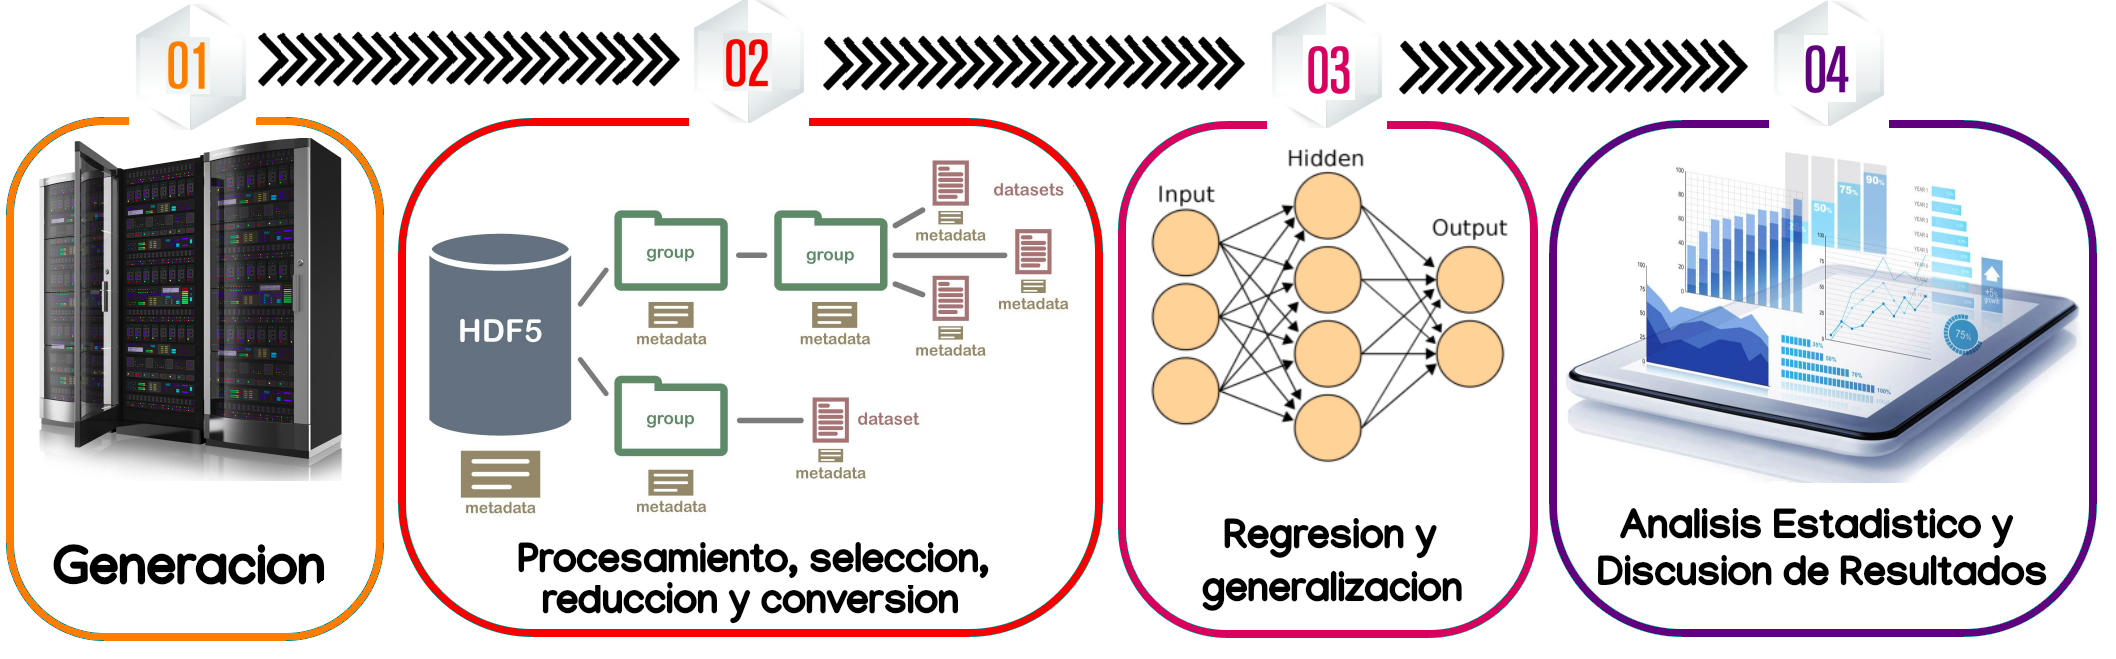
\includegraphics[width=1\textwidth]{Imag/procesos_darksusy.png}
\caption{Secuencia lógica de la investigación.}
\end{figure}

\framebreak

\begin{figure}[h]
\centering
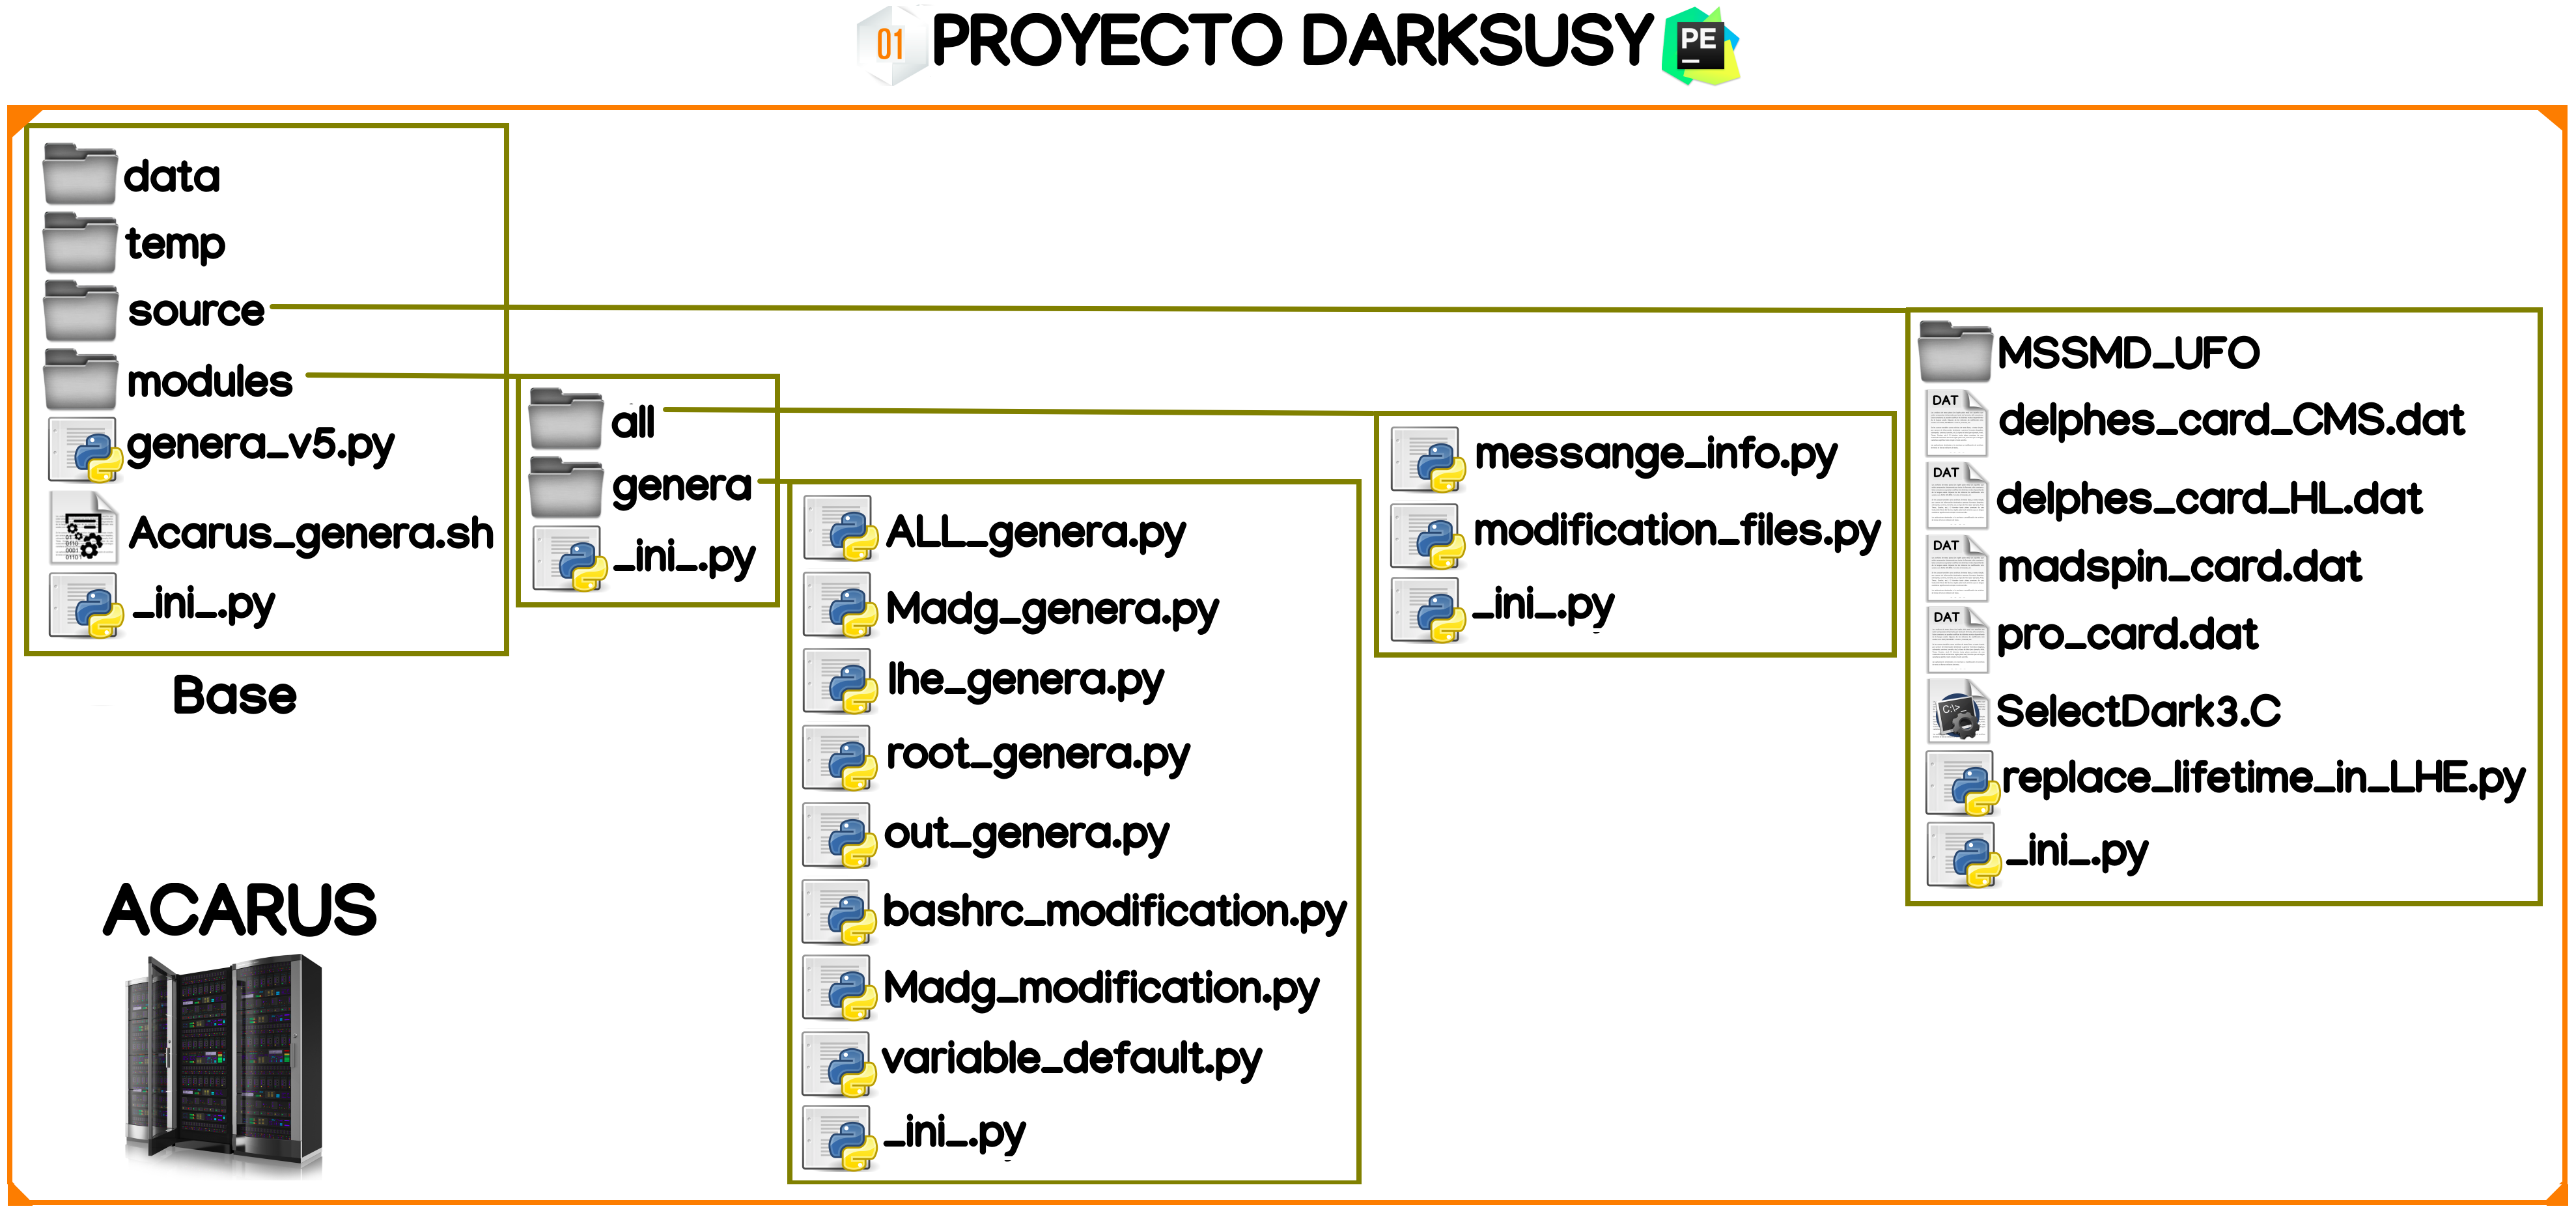
\includegraphics[width=1\textwidth]{Imag/proyecto_darksusy.png}
\caption{Estructura del proyecto generador.}
\end{figure}

\framebreak

\begin{figure}[h]
\centering
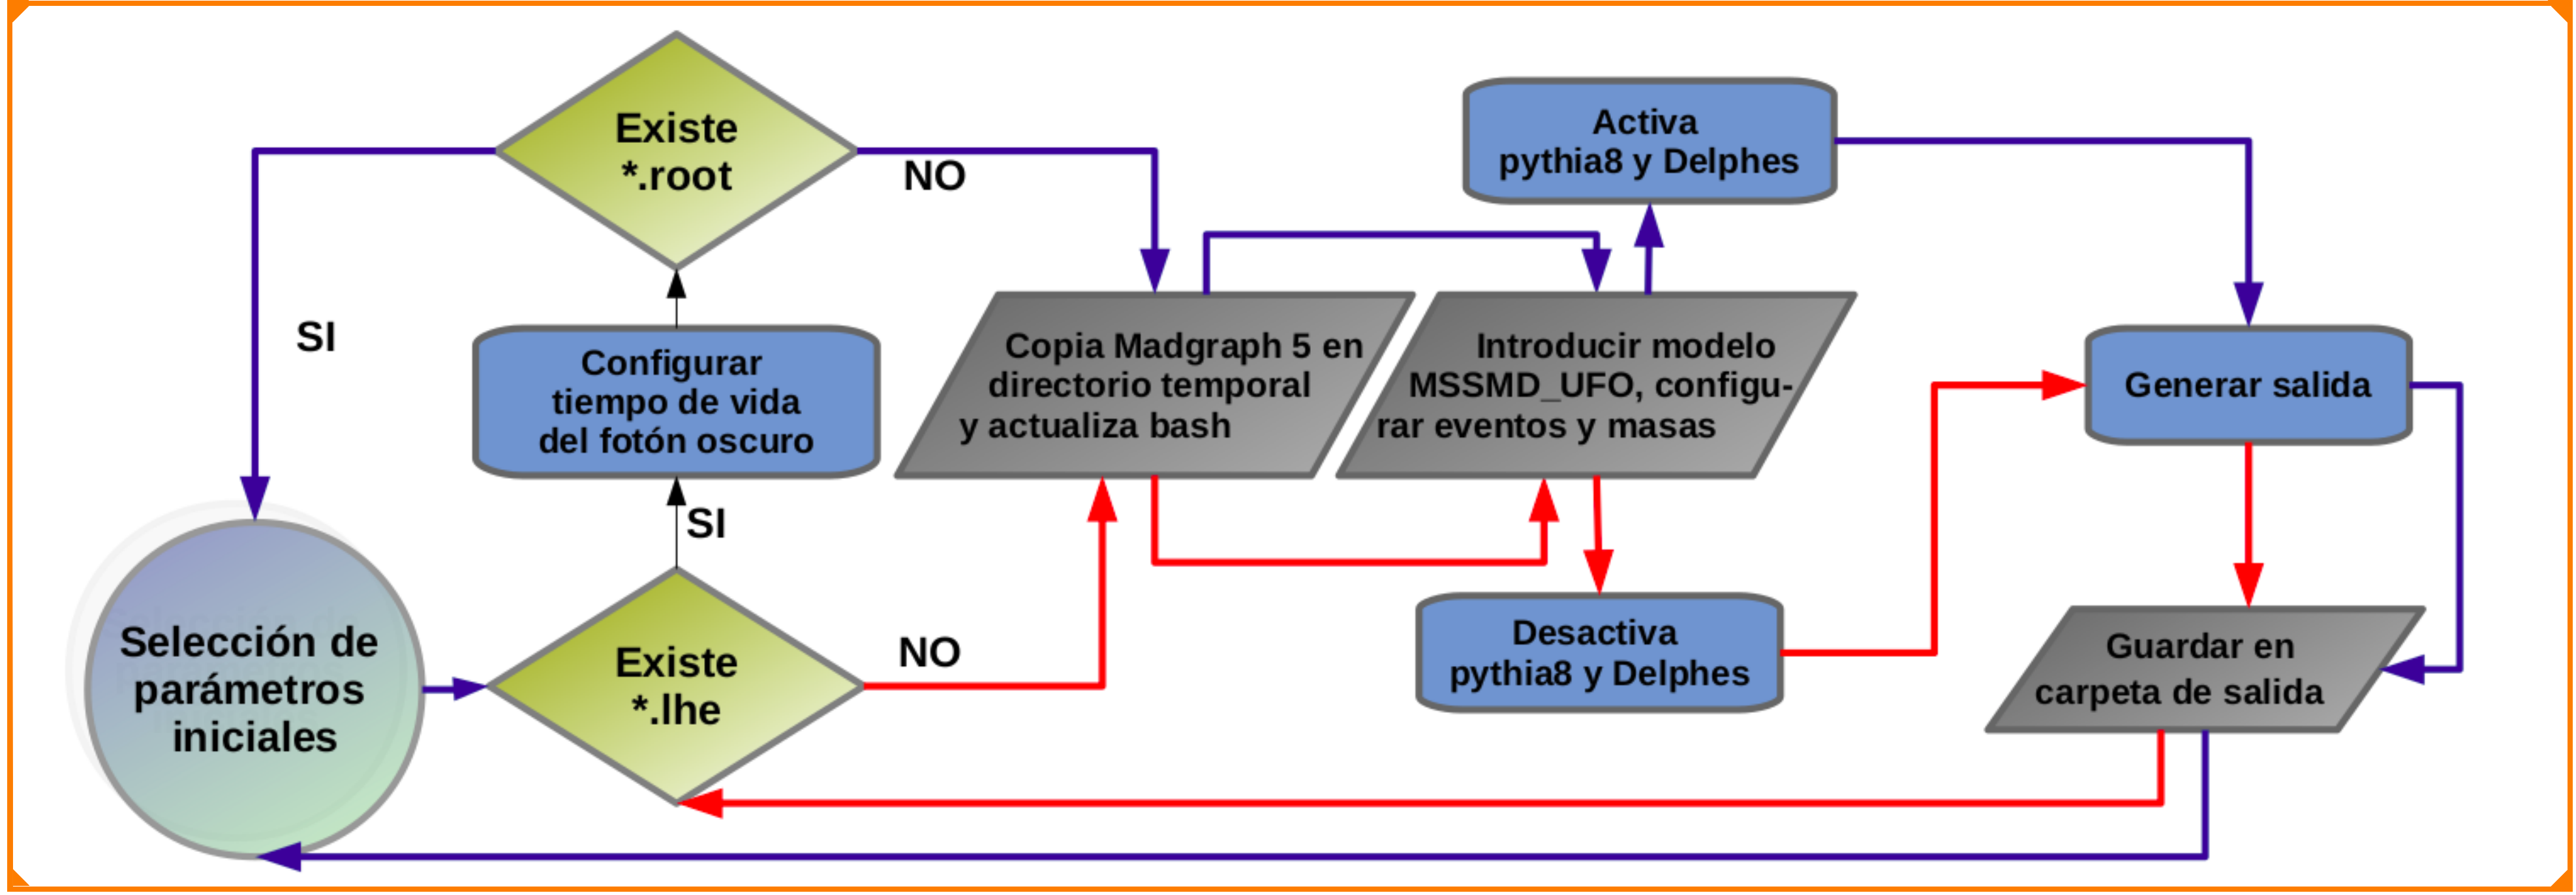
\includegraphics[width=1\textwidth]{Imag/proyecto_darksusy2.png}
\caption{Diagrama de Flujo del generador.}
\end{figure}

\framebreak

\begin{figure}[h]
\centering
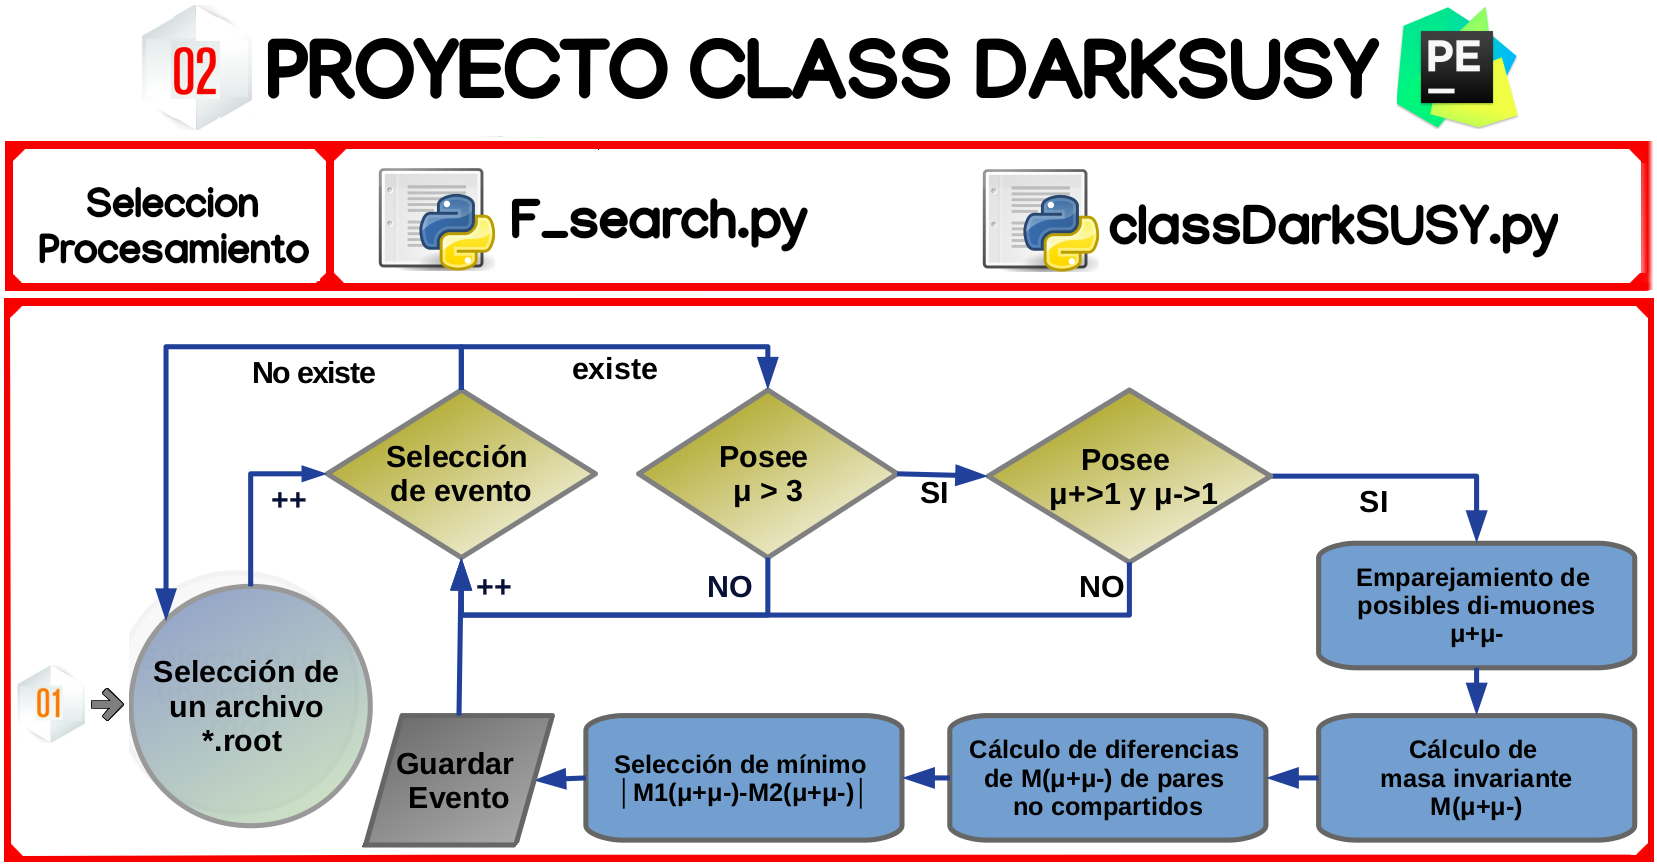
\includegraphics[width=1\textwidth]{Imag/class_darksusy.png}
\caption{Estructura del proyecto interpretador de la información $*.root$.}
\end{figure}

\framebreak

\begin{figure}[h]
\centering
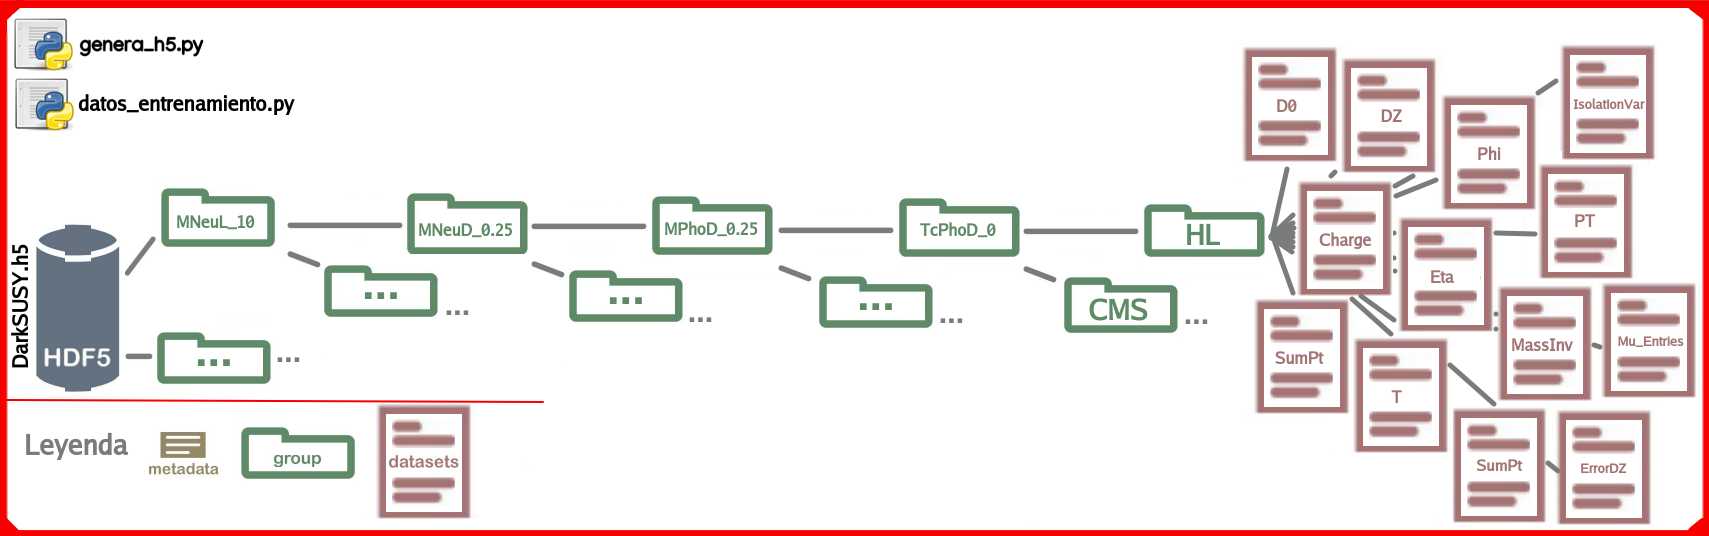
\includegraphics[width=1\textwidth]{Imag/class_darksusy3.png}
\caption{Estructura del archivo h5.}
\end{figure}
\end{frame}



\begin{frame}[fragile,allowframebreaks]{Análisis Preliminar. Análisis del contenido muónico}
\begin{figure}[h]
\centering
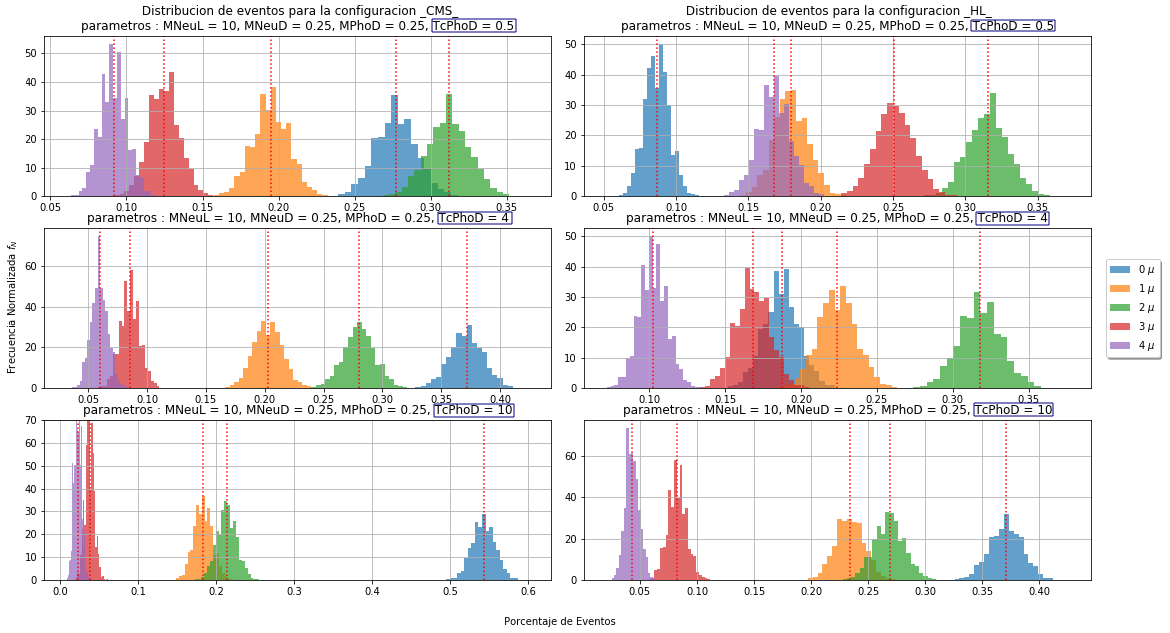
\includegraphics[width=.9\textwidth]{Imag/Distribucion_Entries.png}
\caption{Distribuciones de frecuencia de las entradas $f^{(j,~k)}$ ante cambios de \texttt{TcPhoD}.}
\end{figure}

\framebreak

\begin{figure}[h]
\centering
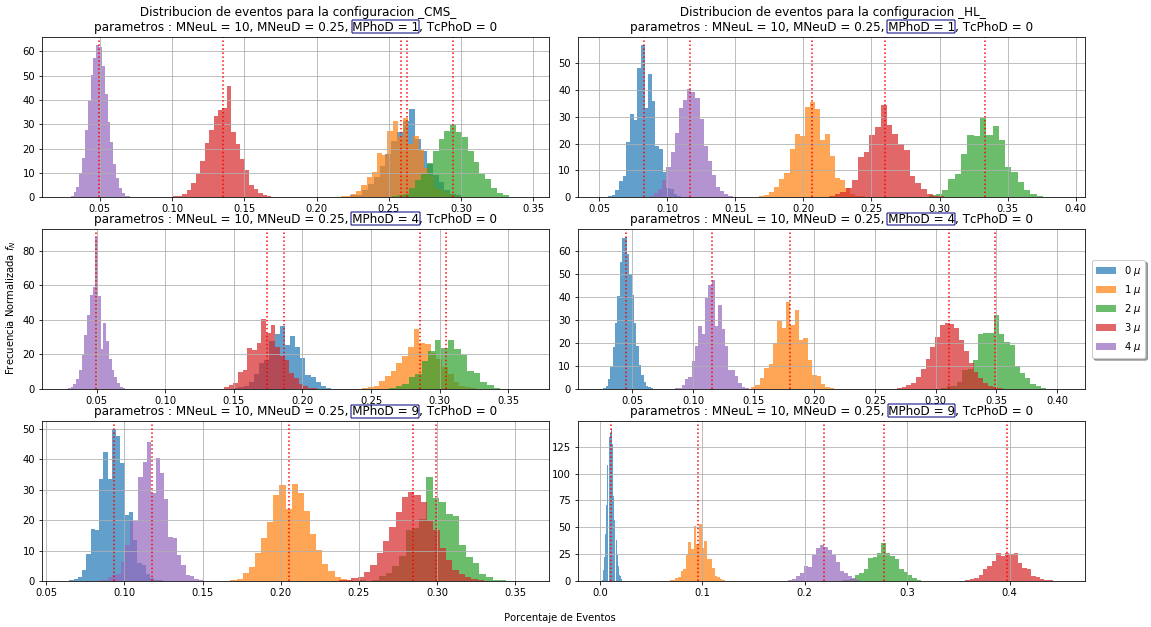
\includegraphics[width=.9\textwidth]{Imag/Distribucion_Entries2.png}
\caption{Distribuciones de frecuencia de las entradas $f^{(j,~k)}$ ante cambios de \texttt{MPhoD}.}
\end{figure}

\framebreak

\begin{figure}[h]
\centering
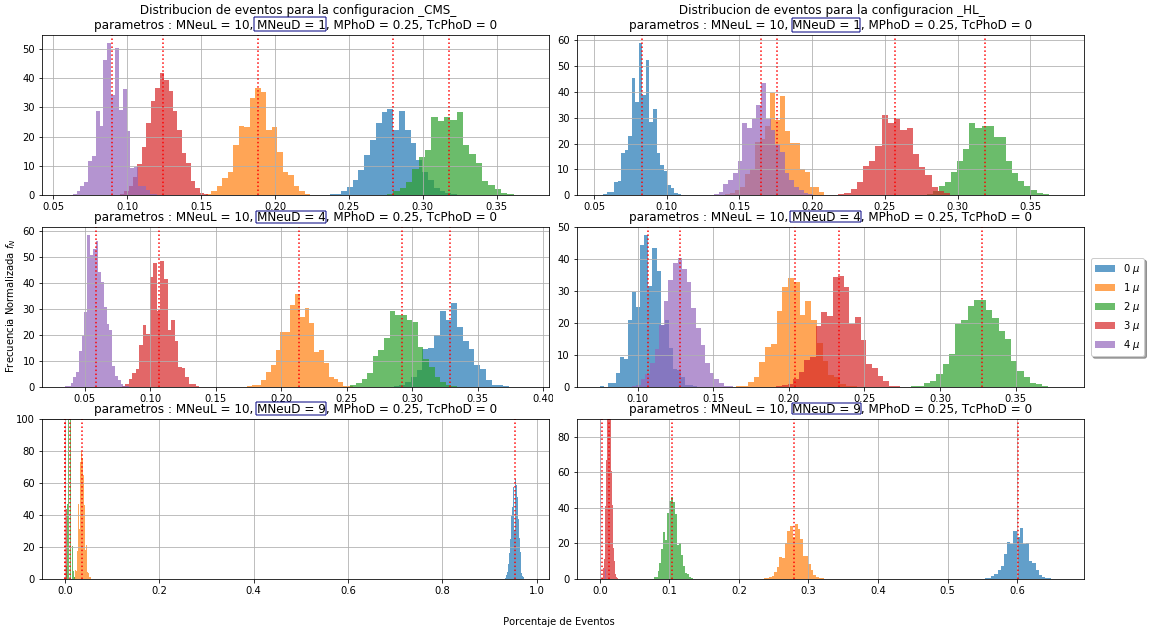
\includegraphics[width=.9\textwidth]{Imag/Distribucion_Entries3.png}
\caption{Distribuciones de frecuencia de las entradas $f^{(j,~k)}$ ante cambios de \texttt{MNeuD}.}
\end{figure}





\end{frame}


\end{document}


